\section{Empirical Results}


\subsection{Sensing Locations for Synthetic Data Sets}\label{sec:exp}
 The goal of this experiment is to investigate the dependency of the observability of system \eqref{k_measure} on the shaded observation matrix and the lower bound presented in Proposition \ref{prop:2}. The domain is fixed on the interval $\dom = [0,2\pi]$. First, we pick sets of points $\shCent^{(\setind)} = \{c_1,\dots,c_{\ncent_{\setind}}\}, \ c_{\centind}\in\dom$, $\ncent=50$, and construct a dynamics matrix $\dualop = \JorLa \in {\R^{\ncent \times \ncent}}$, with cyclic index $5$.  We pick the RBF kernel $\kernel(x,y) = e^{-\|x-y\|^2/2\s^2}$, $\s=0.02$. Generating samples $\sampSet=\sampSetLong$, $x_{\sampind}\in\dom$ randomly, we compute the $\minmeas$-shaded property and observability for this system. Figure \ref{fig:kobs_small} shows how shadedness is a necessary condition for observability, validating Proposition \ref{prop:1}: the slight gap between shadedness and observability here can be explained due to numerical issues in computing the rank of $\Obs_{\Tset}$. 
 
Next, we  consider a system with a cyclic index $\minmeas=18$ to verify random sensor placement results. We constructed the measurement operator $\empK$ using the heuristic in Remark \ref{rem:1} (Algorithm \ref{alg:samples}), and random sensor selection to generate the sampling locations $\sampSet$. These results are presented in Figure \ref{fig:sample_observability}. The plot for random sampling which has been averaged over $ 100 $ runs, resembles a c.d.f function of an exponential distribution $ F(X=x)=1-\exp(-\lambda x) $. This verifies the claim made in Theorem \ref{thm:r2}, as the probability of becoming unobservable decays exponentially with the number of sensors placed. Also, fitting an exponential distribution we found that the mean $ \lambda^{-1}$ comes close to the ratio $ {\rands}/{p} $, which is the expected number of randomly placed sensors required for observability as per Theorem \ref{thm:r1}. Note that observability is not achieved if the number of samples $\nsamp < \minmeas$ verifying the result in Proposition \ref{prop:2}. %, although it is more expensive. 
% Finally, using Algorithm \ref{algo:C2}, we estimate the probable sampling locations $\minmeas $ and check whether the system is observable. We repeat Algorithm \ref{algo:C2}, with $N=\minmeas+1$ and so on, until the system is observable. Figures \ref{fig:aa} and \ref{fig:sample_observability} compares two such results of observability phase transition achieved against an approach that randomly selects sampling locations for $M=50$. Both the plots show that with the random approach we need to sample at more locations as compared to our approach in Algorithm \ref{algo:C2}. Also from the figure \ref{fig:aa}, it is clear that even increasing the number of sampling locations does not guarantee observability for random sampling. %Note that we did not compare with information entropy based methods since they are not applicable 
% For each $M$ the experiment was repeated 100 times; table \ref{sample-table} compares the computed average and variance of sampling locations required to achieve observability using sample locations %$ \hat{c}_{sj} $ 
% from Algorithm \ref{algo:C2} and randomly chosen locations. These results further verify the inference made from figures \ref{fig:aa} and \ref{fig:sample_observability}.
 \vspace{-0.1in}
\subsection{Comparison With Nonstationary Kernel Methods on Real-World Data}\label{sec:comparison}
We use three real-world datasets to evaluate and compare the kernel observer with the two different lines of approach for non-stationary kernels  discussed in Section \ref{sec:related}. For the Process Convolution with Local Smoothing Kernel (PCLSK) and Latent Extension of Input Space (LEIS) approaches, we compare with NOSTILL-GP \cite{garg2012AAAI} and \cite{pfingsten2006nonstationary} respectively, on the Intel Berkeley, Irish Wind and Ozone data-sets. 
% Each of these methods were trained on a particular set of data, and the inferred model was used to perform predictions. 

Model inference for the kernel observer involved three steps: 1) picking the Gaussian RBF kernel $\kernel(x,y) = e^{-\|x-y\|^2/2\s^2}$, a search for the ideal $\s$ is performed for a sparse Gaussian Process model (with a fixed basis vector set $\shCent$ selected using the method in \cite{csato2002sparse}. %\footnote
{For the data set discussed in this section, the number of basis vectors were equal to the number of sensing locations in the training set, with the domain for input set defined over $ \R^2 $}; 2) having obtained $\s$, Gaussian process inference is used to generate weight vectors for each time-step in the training set, resulting in the sequence $\weight_\tindex, \tindex\in\{1,\dots,T\}$; 3) matrix least-squares is applied to this sequence to infer $\dualopApprox$ (Algorithm \ref{alg:egp_trans}). For prediction in the autonomous setup, $\dualopApprox$ is used to propagate the state $\weight_{\tindex}$ forward to make predictions with no feedback, and in the observer setup, a Kalman filter (Algorithm \ref{alg:egp_inf}) with $\nsamp$ determined using Proposition \ref{prop:2}, and locations picked randomly, is used to propagate $\weight_{\tindex}$ forward to make predictions. We also compare with a baseline GP (denoted by `original GP'), which is the sparse GP model trained using all of the available data. 

Our first dataset, the Intel Berkeley research lab temperature data, consists of 50 wireless temperature sensors in indoor laboratory region spanning 40.5 meters in length and 31 meters in width\footnote{\url{http://db.csail.mit.edu/labdata/labdata.html}}. Training data consists of temperature data on March 6th 2004 at intervals of 20 minutes (beginning 00:20 hrs) which totals to 72 timesteps. Testing is performed over another 72 timesteps beginning 12:20 hrs of the same day. Out of 50 locations, we uniformly selected 25 locations each for training and testing purposes. Results of the prediction error are shown in box-plot form in Figure \ref{fig:intel_boxplots} and as a time-series in Figure \ref{fig:intel_comp}, note that `Auto' refers to autonomous set up. Here, the cyclic index of $\dualopApprox$ was determined to be $2$, so $\nsamp$ was set to $2$ for the kernel observer with feedback. Note that here, even the autonomous kernel observer outperforms PCLSK and LEIS overall, and the kernel observer with feedback with $\nsamp = 2$ significantly outperforms all other methods, which is why we did not include results with $\nsamp > 2$. 
% \gXX{explain the significance of N=2, cyclic inde etc, why are we not showing the results with increasing number of feedback locations, include discussion or plots of computational performance, this they will surely ask}
%
%Our first dataset is the well known  Intel Berkeley research lab temperature data. It consists of 50 wireless temperature
%sensors in indoor laboratory region spanning 40.5 meters
%in length and 31 meters in width\footnote{\url{http://db.csail.mit.edu/labdata/labdata.html}}. Training data consisted of temperature data from March 6th 2004 at intervals of  20 minutes (beginning 00:20 hrs) which totals to 72 timesteps. Test was performed over another 72 timesteps beginning 12:20 hrs of the same day. Out of 50 locations, we uniformly
%
%selected 25 locations each for training and testing purposes. For observer, we chose $ \nsamp =2 $ based on the inferred $ \dualopApprox $. For a baseline, we separately train a Gaussian process (for each timestep) assuming knowledge of all data, corresponding result is plotted as ``original". Figure \ref{fig:intel_comp} plots the RMS errors in prediction for each time step, these errors are summarized in the form of box-plots in figure \ref{fig:intel_boxplots}. 




The second dataset is the Irish wind dataset, consisting of daily average
wind speed % (in knots = 0.542 m/s) 
data collected from year
1961 to 1978 at 12 meteorological stations in the Republic
of Ireland\footnote{\url{http://lib.stat.cmu.edu/datasets/wind.desc}}. The prediction error  is in box-plot form in Figure \ref{fig:irish_boxplots} and as a time-series in Figure \ref{fig:irish_comp}. Again, the cyclic index of $\dualopApprox$ was determined to be $2$. In this case, the autonomous kernel observer's performance is comparable to PCLSK and LEIS, while the kernel observer with feedback with $\nsamp = 2$ again outperforms all other methods. 

Finally, the Ozone dataset measures ozone concentration (in parts per billion) measured at 60 stations by the United States Environmental Protection Agency \cite{li2006spatiotemporal} across USA. Due to missing measurements, we only selected data from
year 1997 to 2013 for training and evaluation. For each station, we averaged ozone concentration over a period of three months, resulting in four quarters per year.
Out of 60 sensor locations, we uniformly selected 30 for training and the remaining locations for testing purposes. The prediction error results are presented in box-plot form in Figure \ref{fig:ozone_boxplots} and as a time-series in Figure \ref{fig:ozone_comp}. Here, the cyclic index of $\dualopApprox$ was determined to be $1$. In this case, the performance of autonomous kernel observer is comparable to PCLSK and LEIS, with kernel observer with feedback with $\nsamp = 1$ performing the best. Table \ref{tab:timing} reports the total training and prediction times associated with PCLSK, LEIS, and the kernel observer. We observed that, 1) the kernel observer is an order of magnitude faster than the competing methods, and 2) even for small sets, competing methods did not scale well.

%For both datasets, $ \nsamp =2 $ was chosen based on the inferred $ \dualopApprox $ using proposition \ref{prop:2}. In both cases the cyclic index of $ \dualopApprox $ was one. We also investigated prediction errors for chosing sampling locations randomly from the training set. For this we performed 100 runs of experiment, and the results are shown in Table 1. This empirical evidence shows that it suffices to randomly select sampling/sensing locations for Kernel Observer. 
\begin{table}[h]
	\centering
	\caption{Total training and prediction times for Figs. \ref{intel} and \ref{irish} } \label{tab:timing}
		\begin{tabular}{c|ccc}
		\toprule
			{\bf }  & {\bf Intel } & {\bf Irish } &  {\bf Ozone}  \\
			& Berkeley & Wind & \\
			\midrule
			\emph{Data Size}        & 25-72 & 12-36  & {30-68} \\ 
		    (\emph{bases}-\emph{timesteps})                 &       & & \\ \hline
			Kernel Observer         & 2.1 sec & 0.1 sec & 1.61 sec \\
			PCLSK             & 121.4 sec & 7.0 sec & 91.90 sec \\
			LEIS             & 43.8 sec & 2.8 sec & 37.41 sec\\
		\bottomrule
		\end{tabular}
\end{table}
\vspace{-0.1in}
\subsection{Prediction of Global Ocean Surface Temperature}\label{sec:avhhr}
We analyzed the feasibility of our approach on a very large dataset from the National Oceanographic Data Center: the $4$ km AVHRR Pathfinder project, which is a satellite monitoring global ocean surface temperature (Figure \ref{fig:Rawpathfinder} shows raw satellite data). This dataset is challenging, with measurements at over $37$ million possible coordinates, but with only around 3-4 million measurements available per day, leading to a lot of missing data. The goal was to learn the day and night temperature models on data from the year 2011, and then to monitor  thereafter for 2012. Success in monitoring would demonstrate two things: 1) the modeling process can capture spatiotemporal trends that generalize across years, and 2) the observer framework allows us to infer the state using a number of measurements that are an order of magnitude fewer than available. Note that due to the size of the dataset and the high computational requirements of the nonstationary kernel methods, a comparison with them was not pursued. To build the autonomous kernel observer and general kernel observer models, we followed the same procedure outlined in Section \ref{sec:comparison}, but with $\shCent=\shCentLong$, $c_{\centind}\in\R^{2}, \ |\shCent| = 300$. The Kalman filter for the general kernel observer model  used $\nsamp \in \{250,500,1000\}$ at random locations to track the system state given a random initial condition $\weight_0$. As a fair baseline, the observers are compared to training a sparse GP model (labeled `original')  on approximately $400,000$ measurements per day. %, to get a fair comparison. 
Figure \ref{fig:pathfinder} is an estimate of global ocean surface temperatures obtained using autonomous kernel observer.
Figures \ref{fig:time_series_day} and \ref{fig:time_series_night} compare the autonomous and feedback approach with $1,000$ samples to the baseline GP; here, it can be seen that the autonomous does well in the beginning, but then incurs an unacceptable amount of error when the time series goes into 2012, i.e. where the model has not seen any training data, whereas FKO does well throughout. 
Figures \ref{fig:pathfinder_errors_boxplots_day} and \ref{fig:pathfinder_errors_boxplots} show a  comparison of the RMS error of estimated values from the real data.
This figure shows the trend of the observer getting better and better state estimates as a function of the number of sensing locations $\nsamp$ \footnote{Note that we checked the performance of training a GP with only $1,000$ samples as a control, but the average error was about 10 Kelvins, i.e. much worse than FKO.}.
 Time required for kernel observer is much lesser than retraining the model every time step, see figures \ref{fig:pathfinder_tr_times_boxplots_day}-\ref{fig:pathfinder_tr_times_boxplots_night}.
 
 \textbf{Weather Anomaly in 2012:} We further investigated the poor performance of autonomous kernel observer in the year 2012 as observed in Figures \ref{fig:time_series_day} and \ref{fig:time_series_night}. Clearly, the error in prediction blows up at the start of May in the year 2012. Indicating that the autonomous model trained using the data of the year 2011 does well in capturing the annual weather dynamics up to the month of May 2012. We turned our attention towards the weather in May 2012, as changes in ocean temperatures are directly related to the weather. Surprisingly, severe weather onset was reported on the east coast of United States in May 2012, and this anomaly continued over the period of May to June 2012. Thus, the apparent poor performance of autonomous kernel observer can actually be a useful indicator in detecting the anomalous behavior, as was the case with the ocean temperature in May 2012 which had deviated from the nominal weather dynamics observed in the year 2011 in which no severe weather anomalies were reported. Further, we identified the locations at which the prediction error was two standard deviations above the mean error. These error locations are plotted in Figure \ref{fig:anomaly}. Error locations on 6-7th May coincide with the severe weather onset on the east coast of United states and that of 28-29th May were along the track of storm Beryl approaching the eastern coastline. This shows that the autonomous kernel observer model captures the dynamics of spatiotemporal evolution, and has the potential of identifying current behavior as anomalous to that observed in the training set.
 
\begin{figure}
\centering
    \subfloat[Shaded vs. observability]
    {
    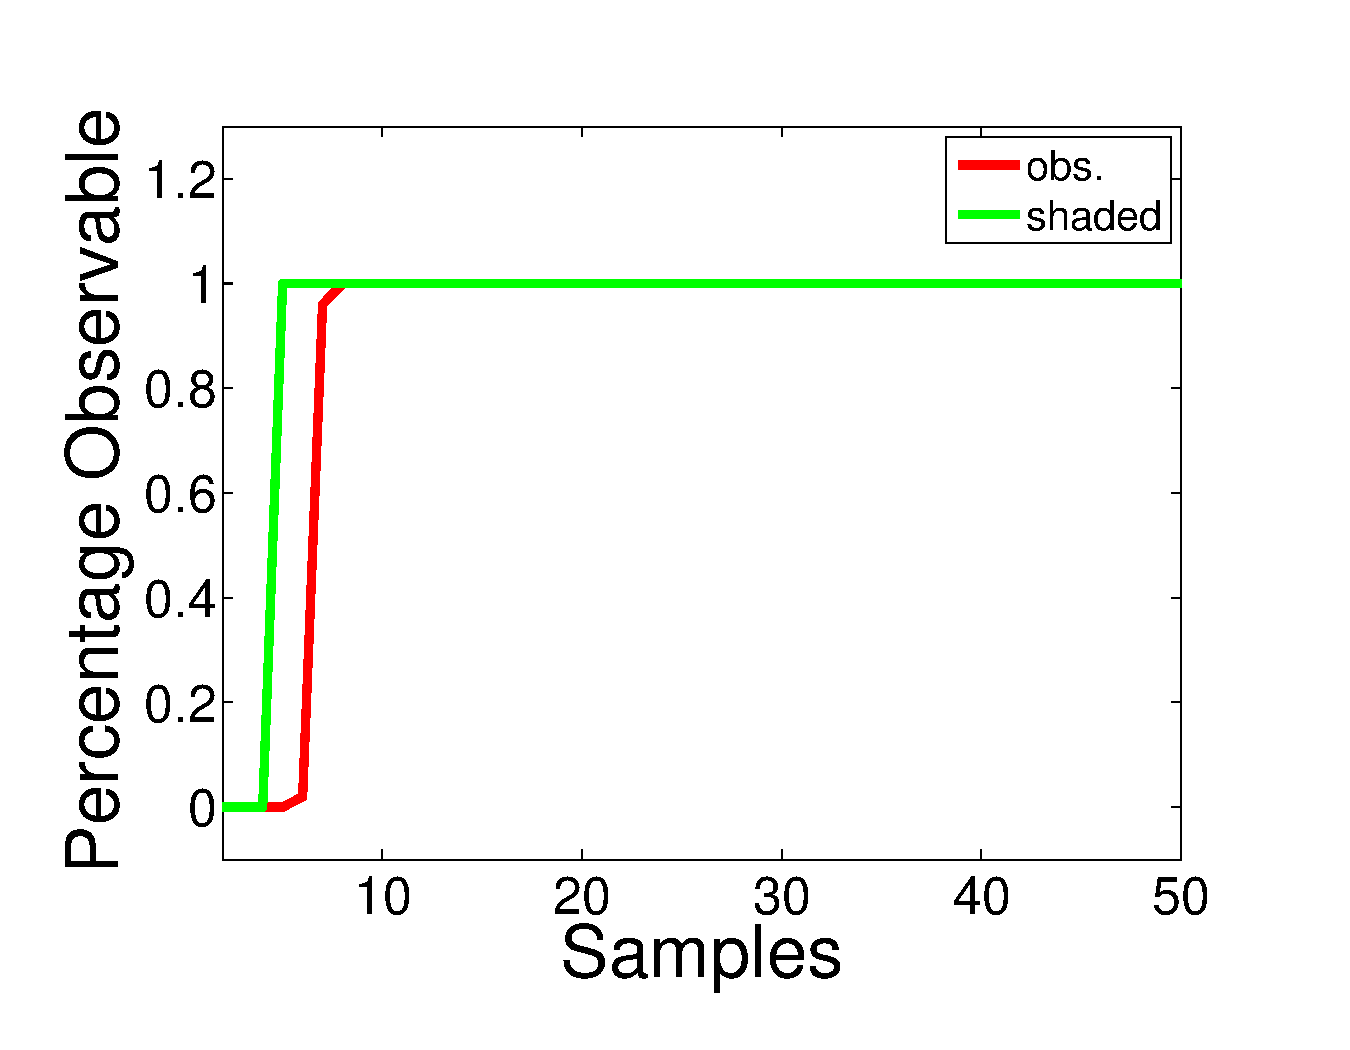
\includegraphics[width=0.45\columnwidth]{kernel_observer_50_cents_smooth4_bandwidth_small.pdf}
    \label{fig:kobs_small}}
     \subfloat[Heuristic vs. random]
     {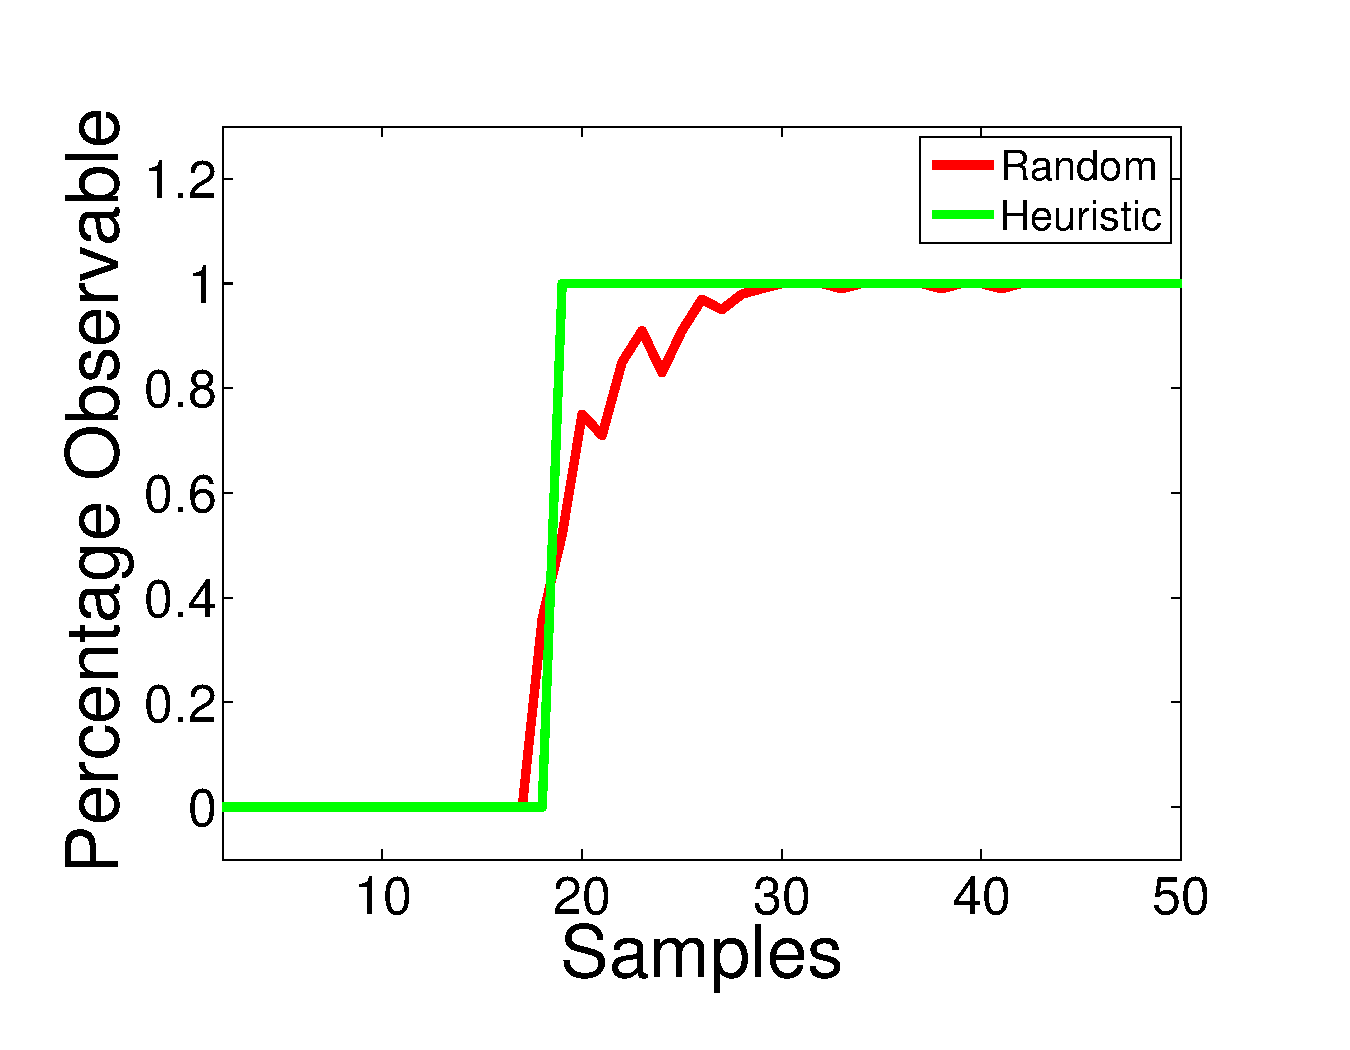
\includegraphics[width=0.45\columnwidth]{rand_average.pdf}
     \label{fig:sample_observability}}  
    \caption{Kernel observability results.}
%\end{figure}
%\begin{figure}[tbh] %{r}{0.5\textwidth}
\end{figure} 

\begin{figure}
\centering
\begin{minipage}{0.48\textwidth}
	% \begin{center}
	\centering
	\subfloat[Error (boxplot)]{
		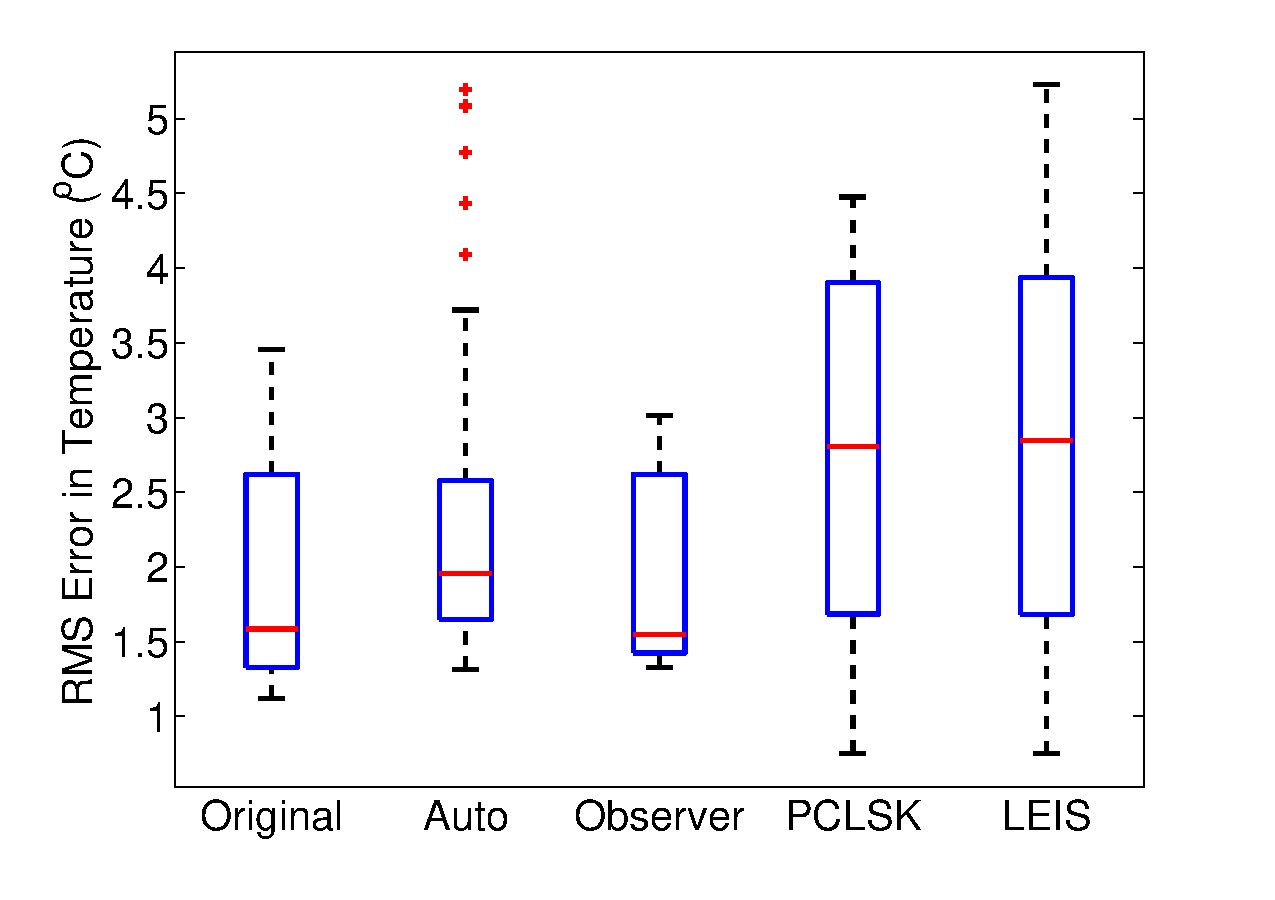
\includegraphics[width=0.45\columnwidth]{box_plot_intel} \label{fig:intel_boxplots} } %pathfinder_errors_boxplot_2012_all_models_night.pdf
	\subfloat[Error (time-series)]
	{
		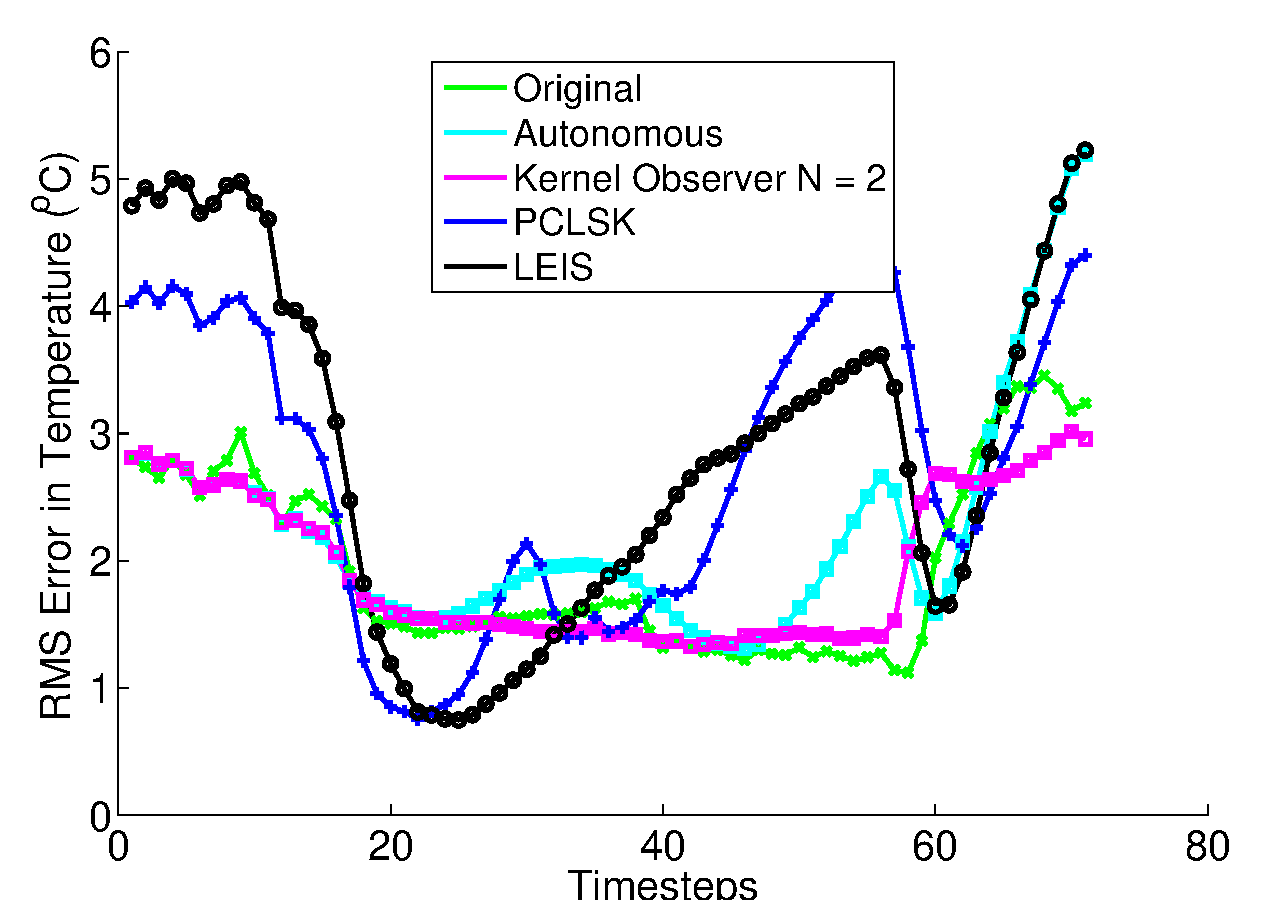
\includegraphics[width=0.45\columnwidth]{Intel_comp} \label{fig:intel_comp}}
	\caption{Comparison of kernel observer to PCLSK and LEIS methods on Intel Berkeley dataset.}     \label{intel}
\end{minipage}
\begin{minipage}{0.48\textwidth}
	
		\subfloat[Error (boxplot)]{
		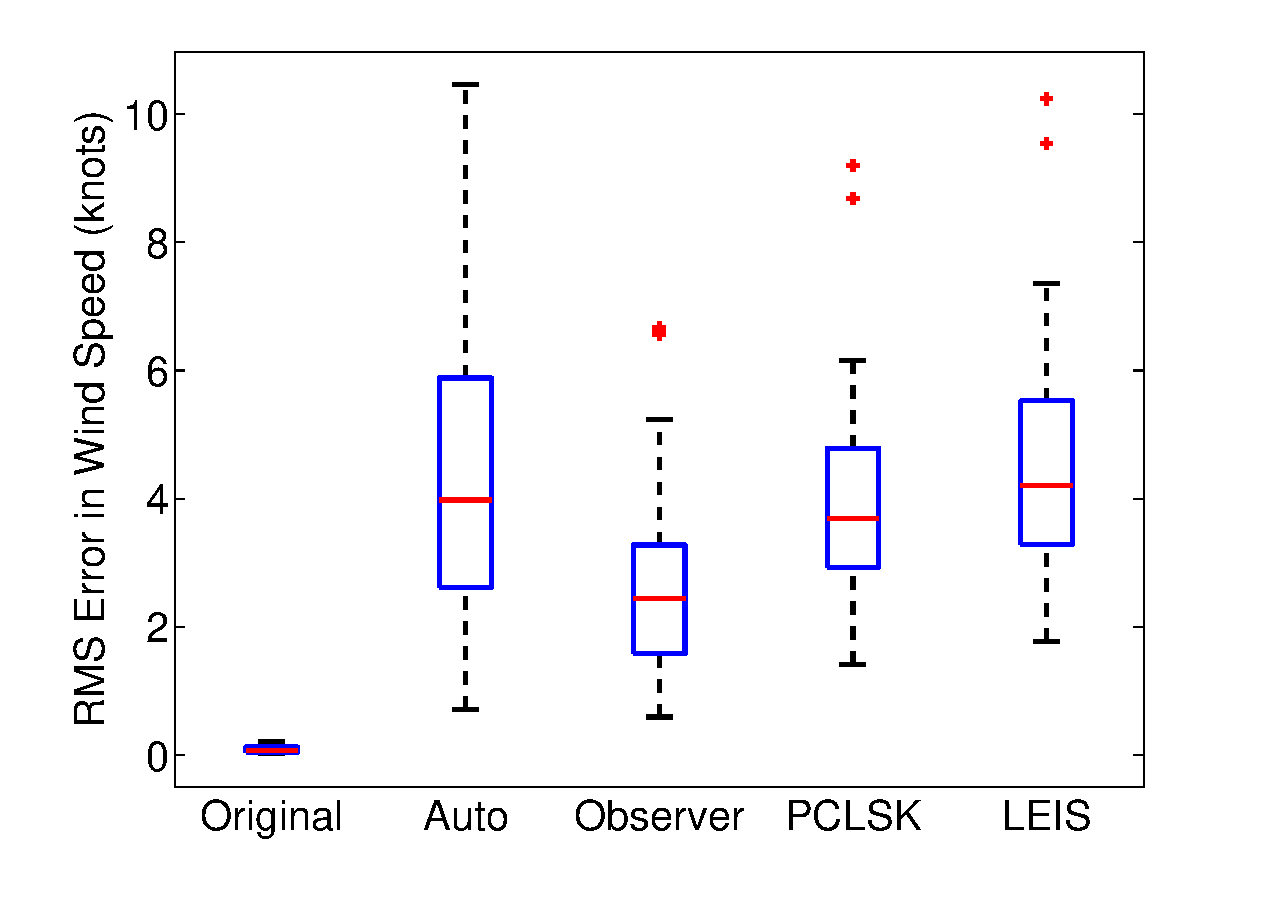
\includegraphics[width=0.45\columnwidth]{box_plot_irish} \label{fig:irish_boxplots} }
		\subfloat[Error (time-series)]{
			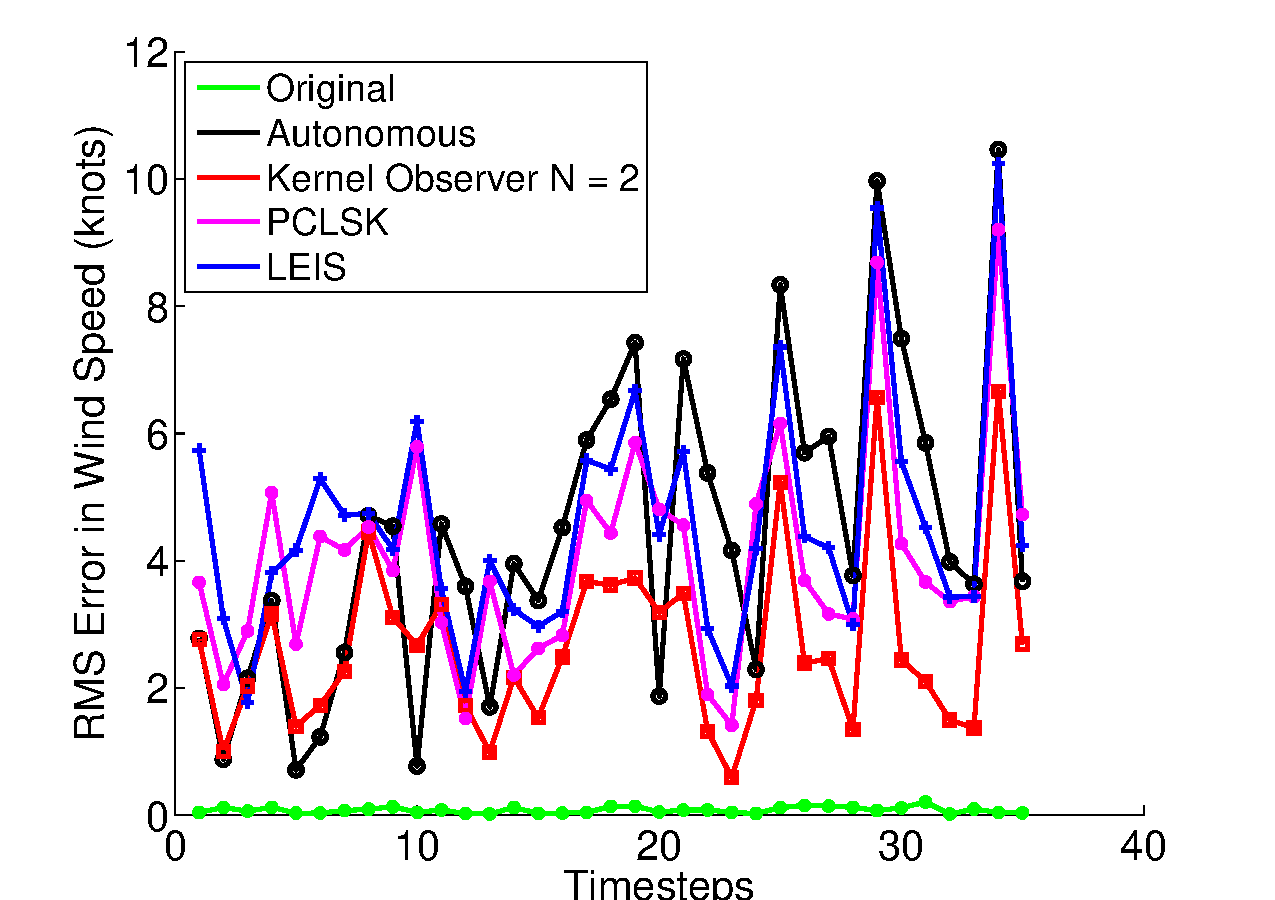
\includegraphics[width=0.45\columnwidth]{irish_wind_comp} \label{fig:irish_comp} }
		\caption{Comparison of kernel observer to PCLSK and LEIS methods on Irish Wind dataset.}\label{irish}
\end{minipage}
\begin{minipage}{0.48\textwidth}
	
		\subfloat[Error (boxplot)]{
		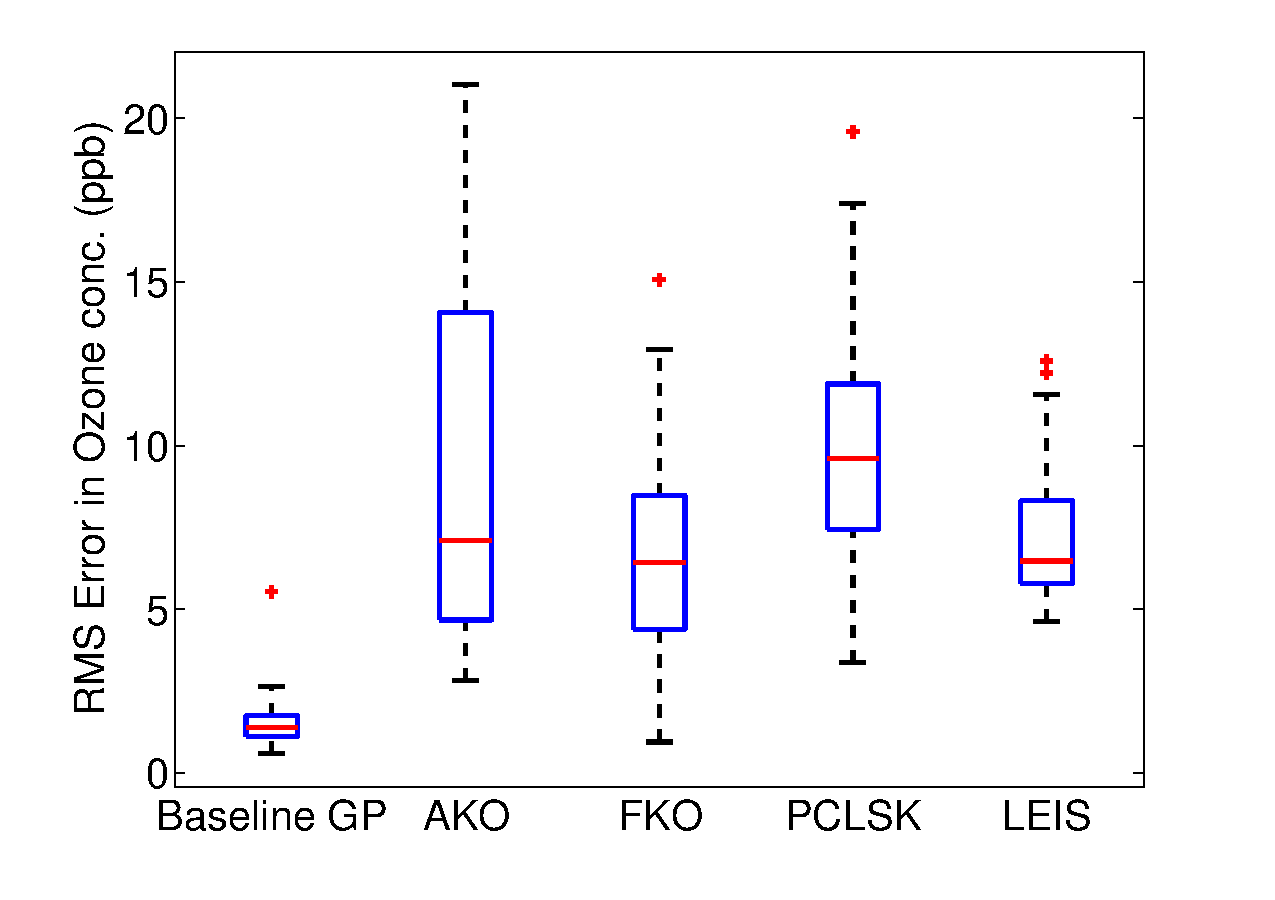
\includegraphics[width=0.45\columnwidth]{box_plot_ozone} \label{fig:ozone_boxplots} }
		\subfloat[Error (time-series)]{
			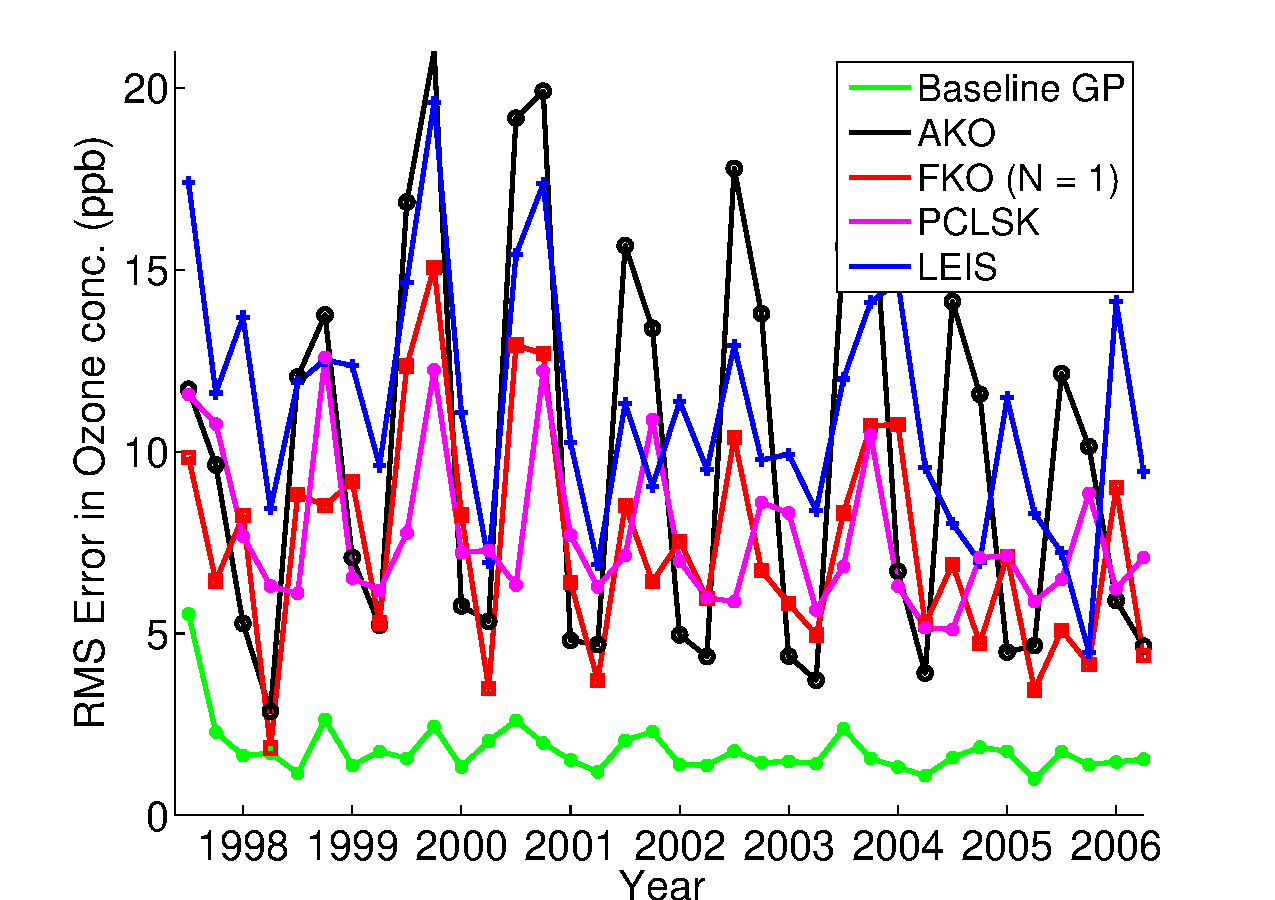
\includegraphics[width=0.45\columnwidth]{ozone_time_series} \label{fig:ozone_comp} }
		\caption{Comparison of kernel observer to PCLSK and LEIS methods on Irish Wind dataset.}\label{ozone}
\end{minipage}
\end{figure}
\begin{figure}
	\centering
	\subfloat[Raw Satellite Data]{
	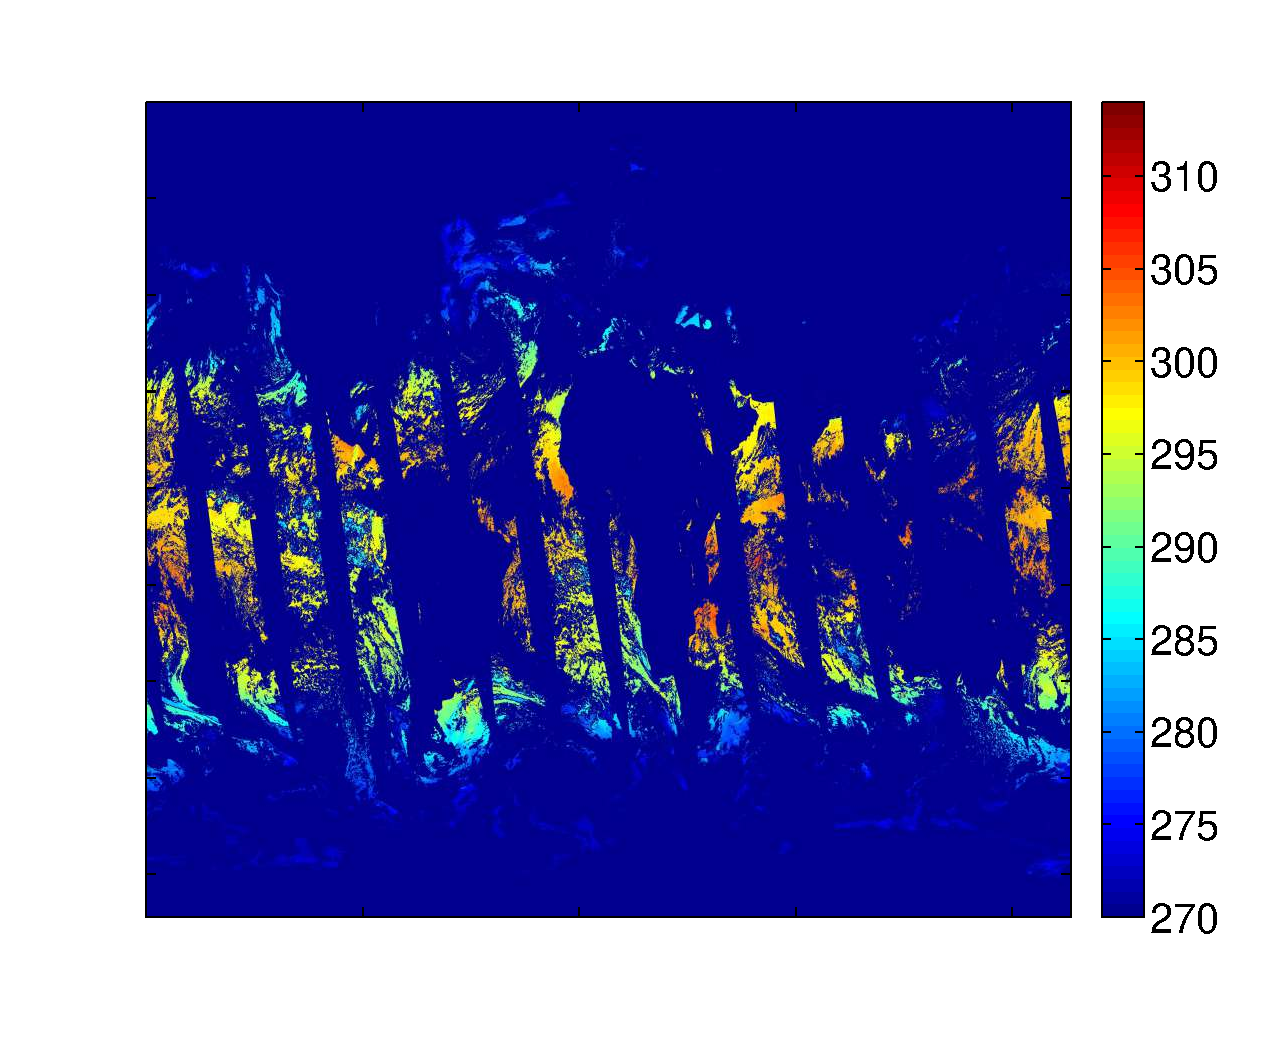
\includegraphics[width=0.4\columnwidth]{pathfinder_raw_data_example}
	\label{fig:Rawpathfinder} }
	\subfloat[AKO estimate]{
	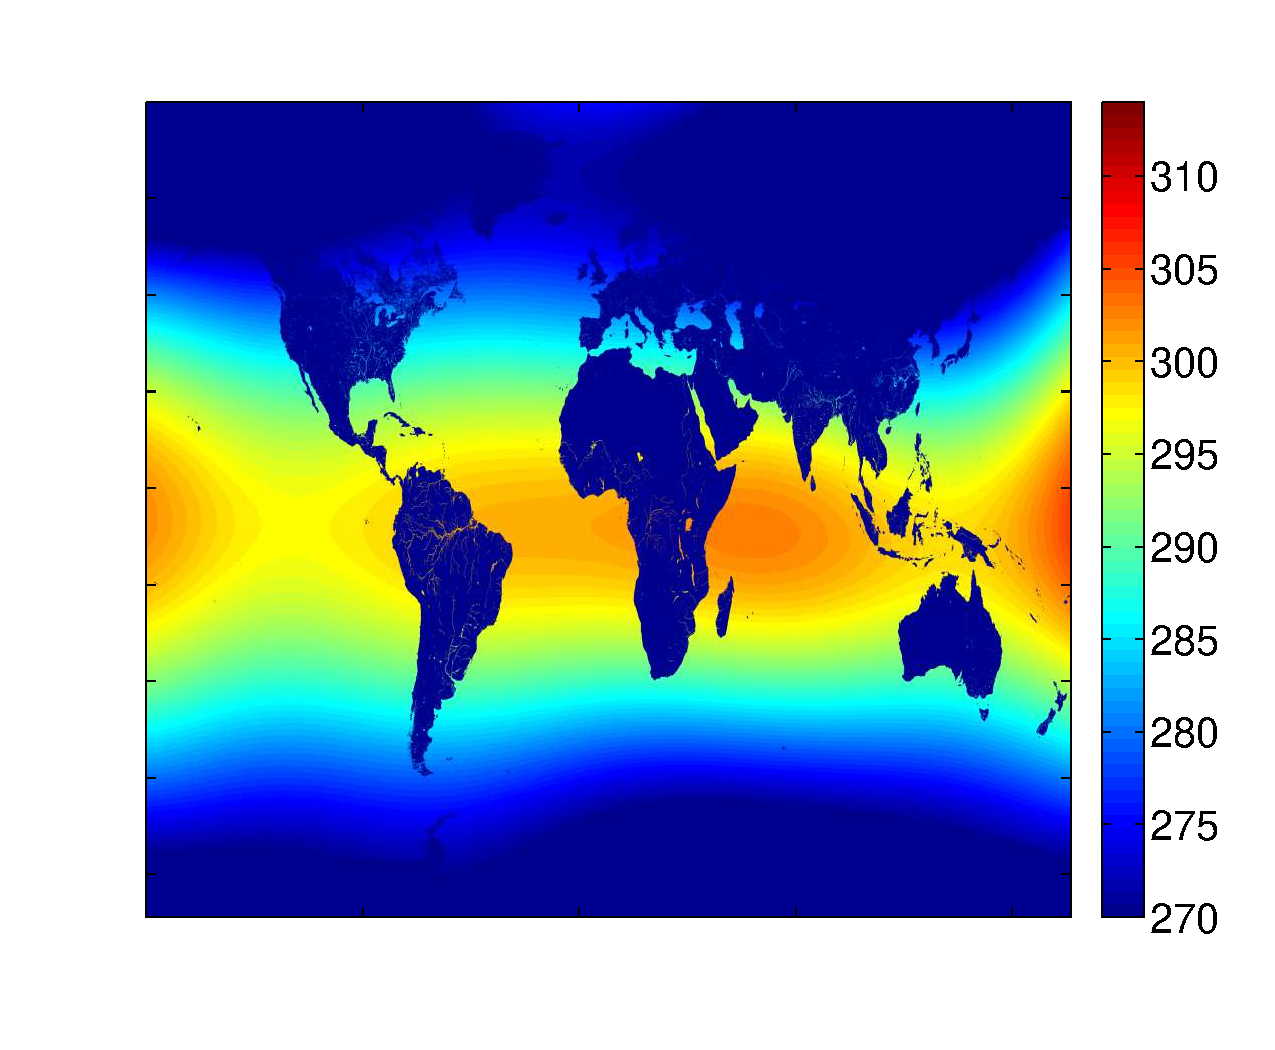
\includegraphics[width=0.4\columnwidth]{pathfinder_inference_example}
	\label{fig:pathfinder} }
	
	\subfloat[Error-day (time-series)]{
		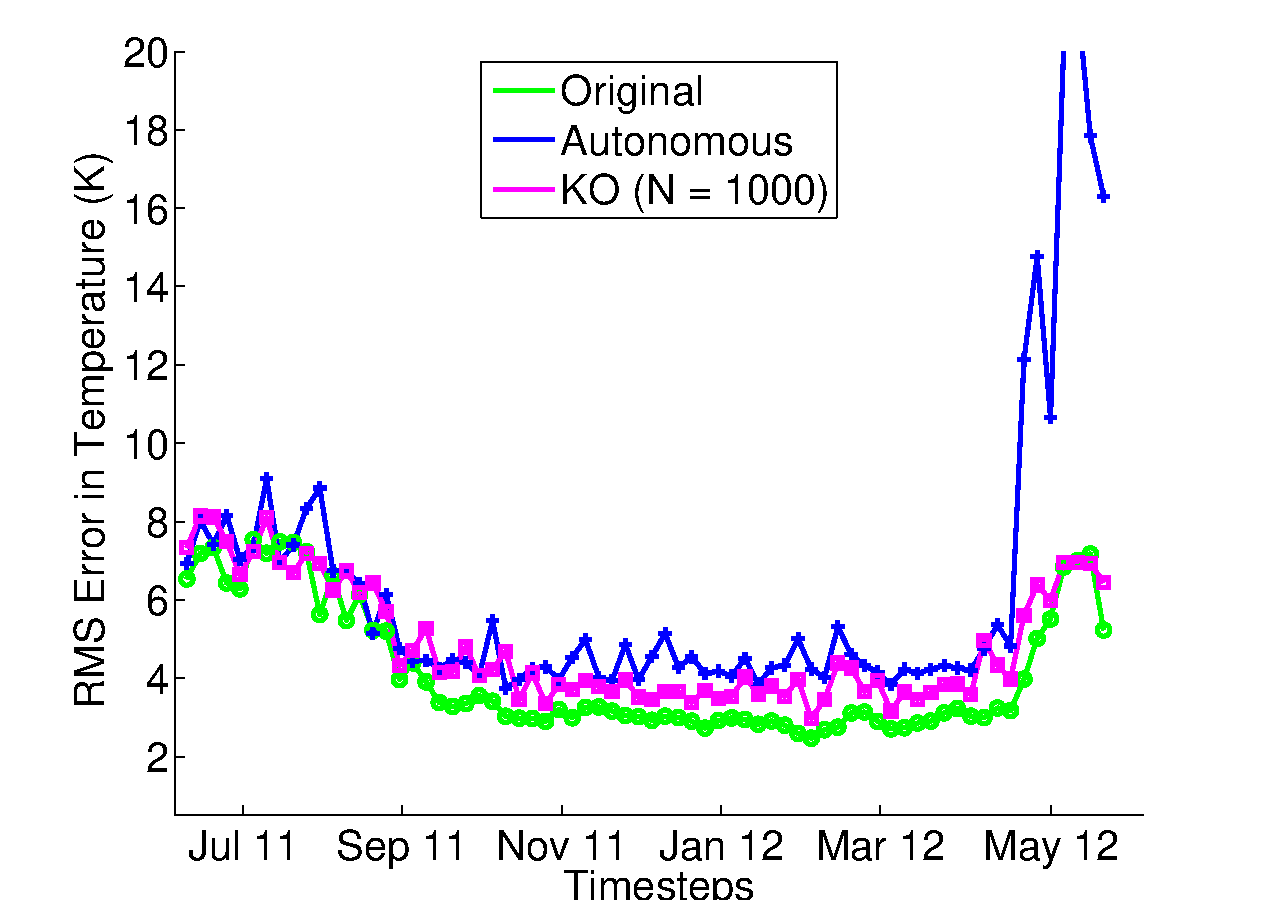
\includegraphics[width=0.4\columnwidth]{time_series_day} \label{fig:time_series_day} }
	\subfloat[Error-night (time-series)]{
		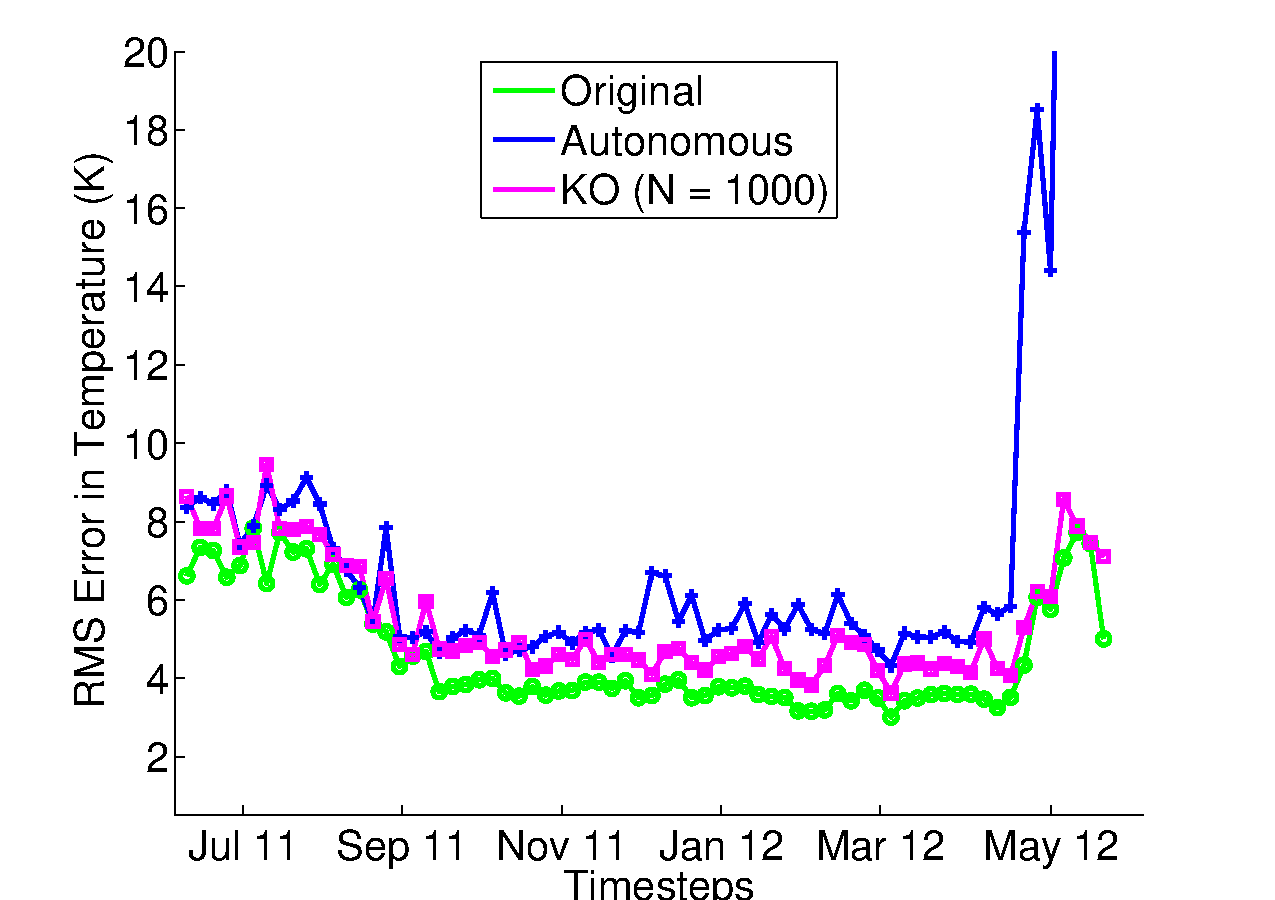
\includegraphics[width=0.4\columnwidth]{time_series_night} \label{fig:time_series_night} }
	 %pathfinder_errors_boxplot_2012_all_models_night.pdf
	 
	\subfloat[Error-day (box-plot)]{
		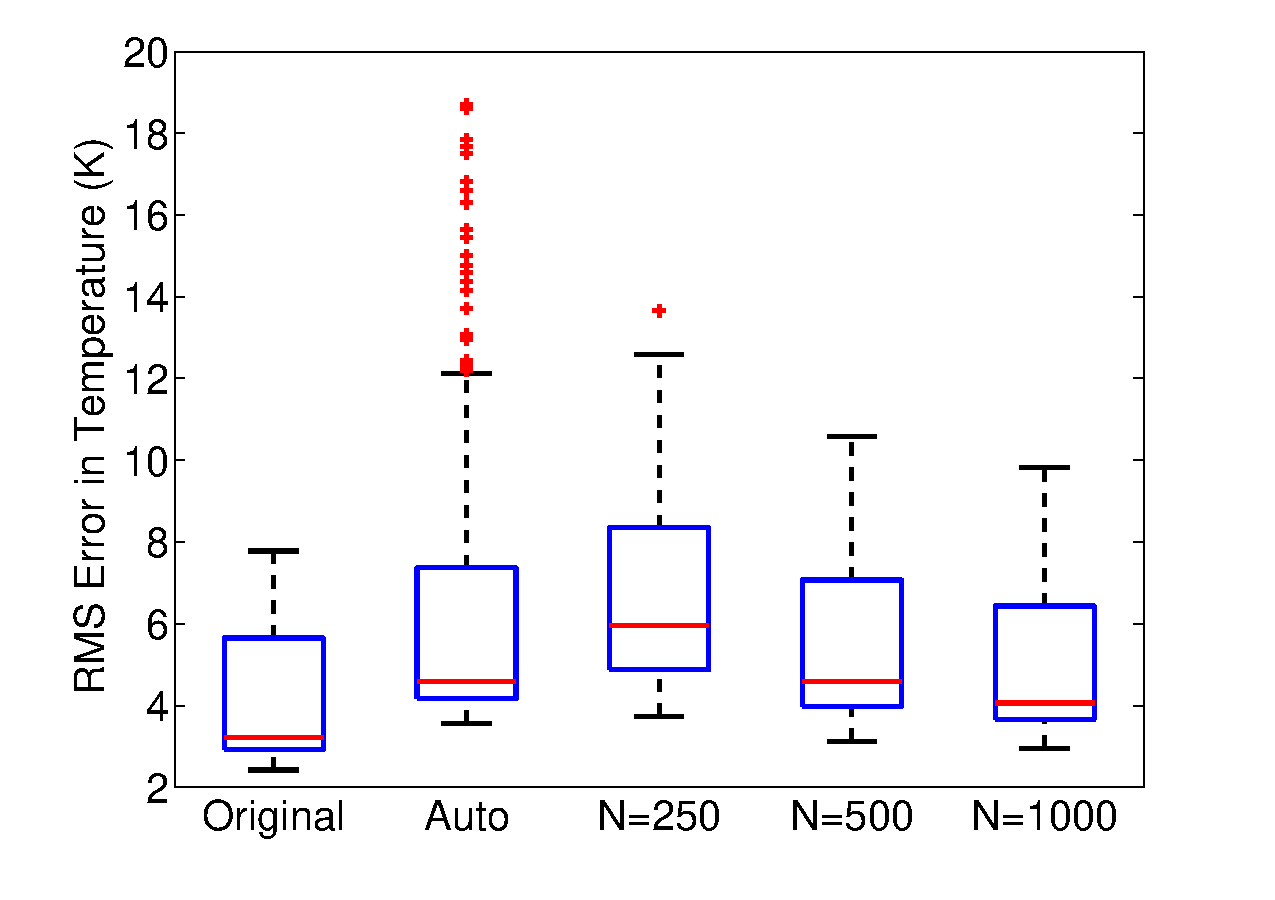
\includegraphics[width=0.4\columnwidth]{box_plot_path_day} \label{fig:pathfinder_errors_boxplots_day} }
	\subfloat[Error-night (box-plot)]{
		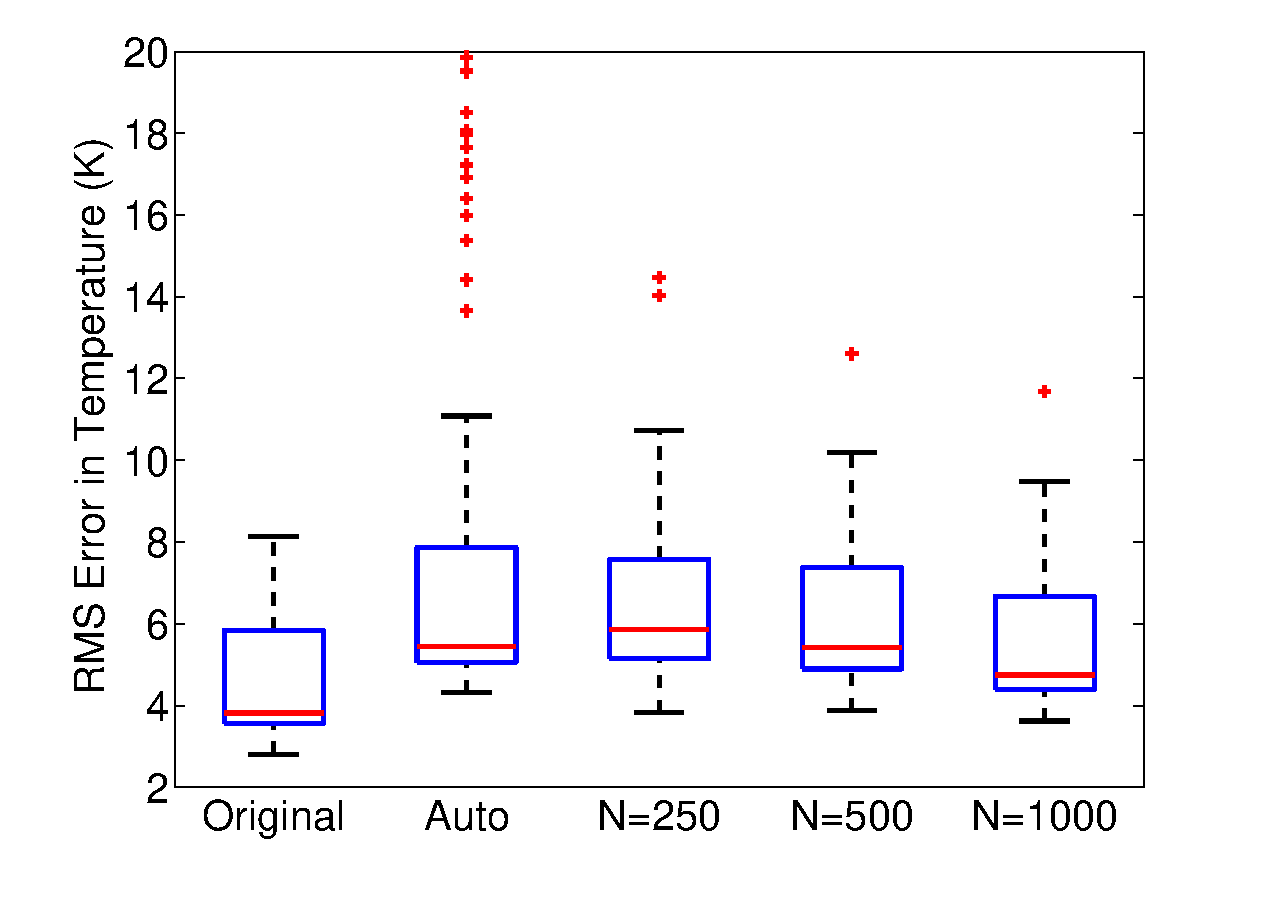
\includegraphics[width=0.4\columnwidth]{box_plot_path} \label{fig:pathfinder_errors_boxplots} }
		
	\subfloat[Estimation time (day)]
	{
		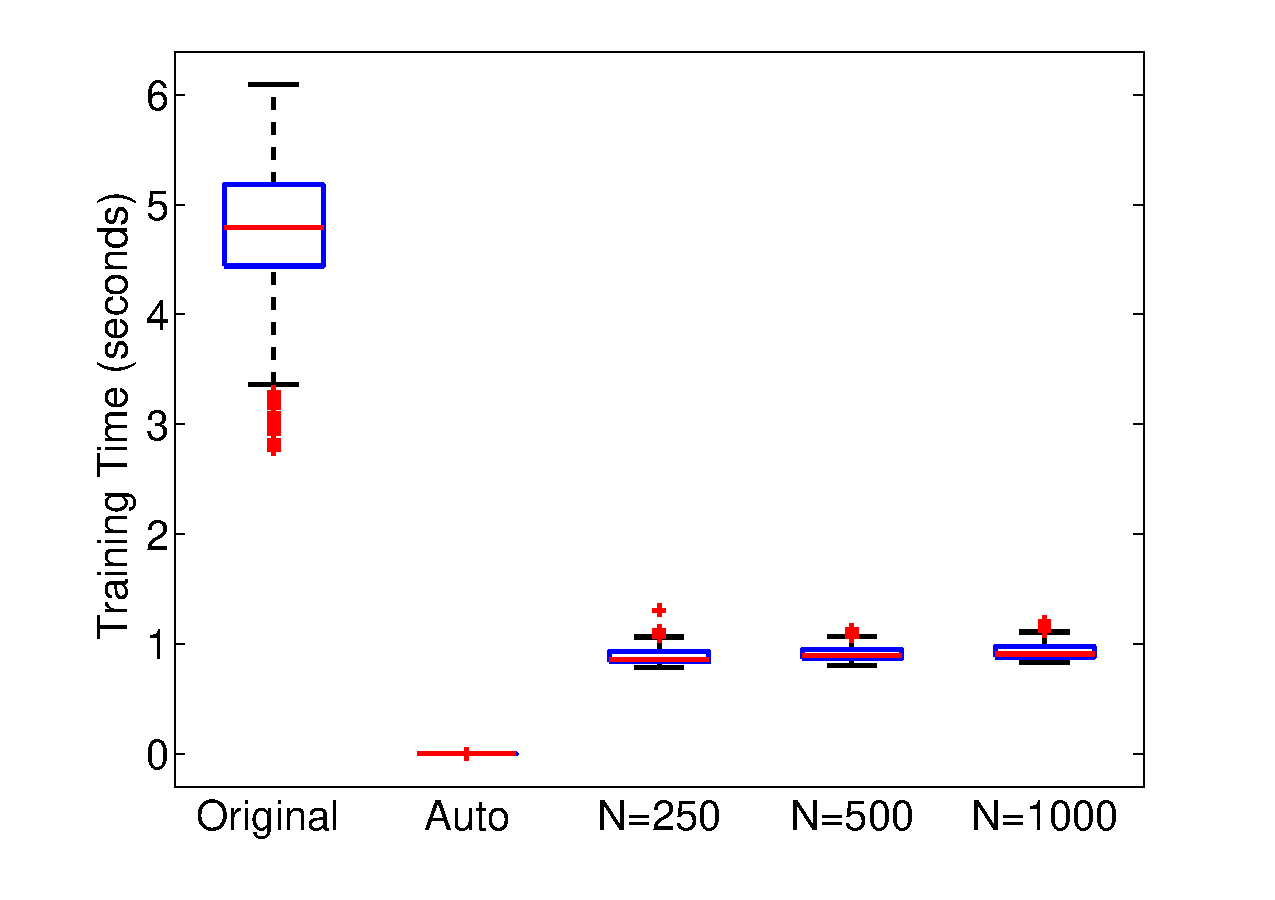
\includegraphics[width=0.4\columnwidth]{box_plot_path_day_time} \label{fig:pathfinder_tr_times_boxplots_day}}
	\subfloat[Estimation time (night)]
	{
		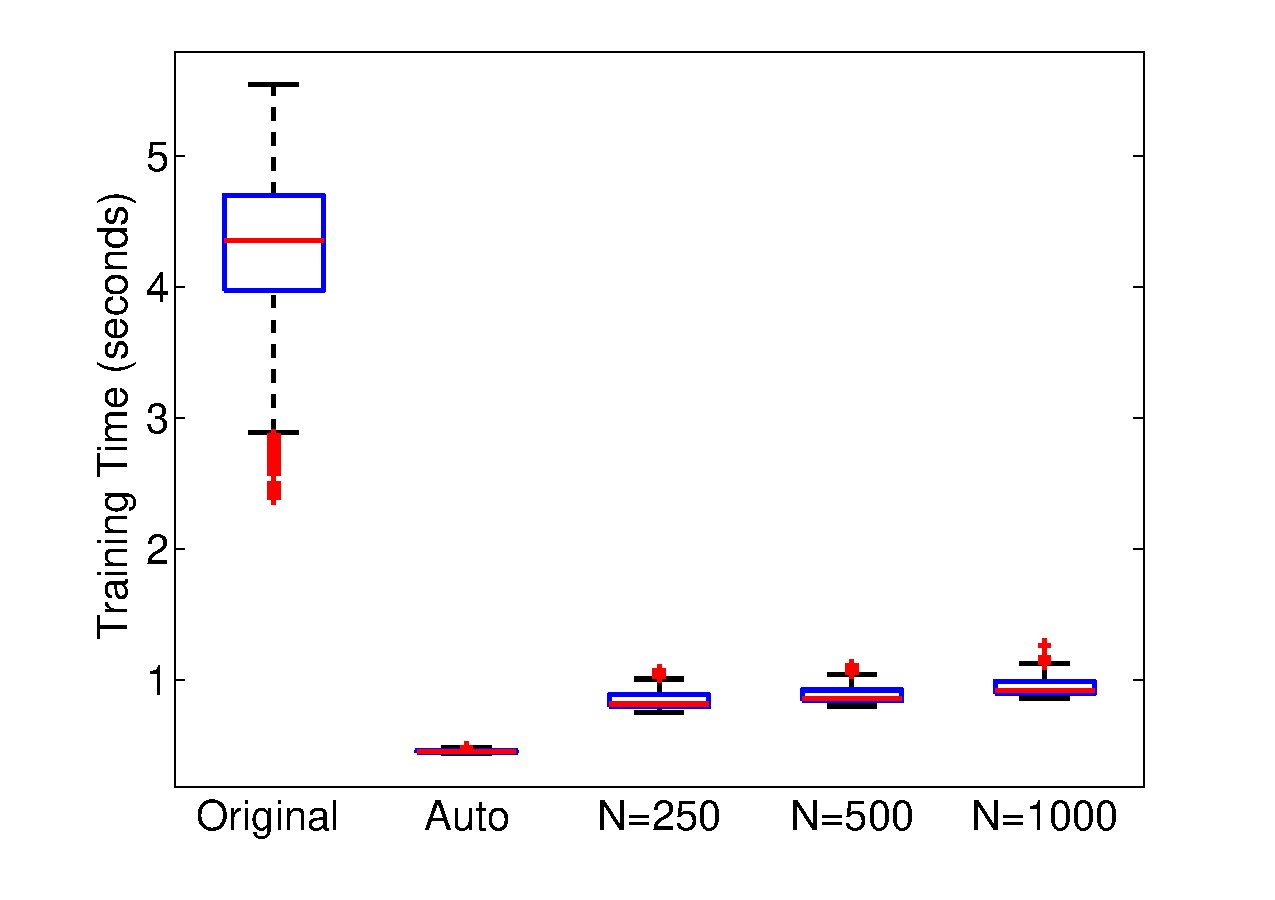
\includegraphics[width=0.4\columnwidth]{box_plot_path_time} \label{fig:pathfinder_tr_times_boxplots_night}}
		
%	\subfloat[Estimation time (night)]
%	{
%		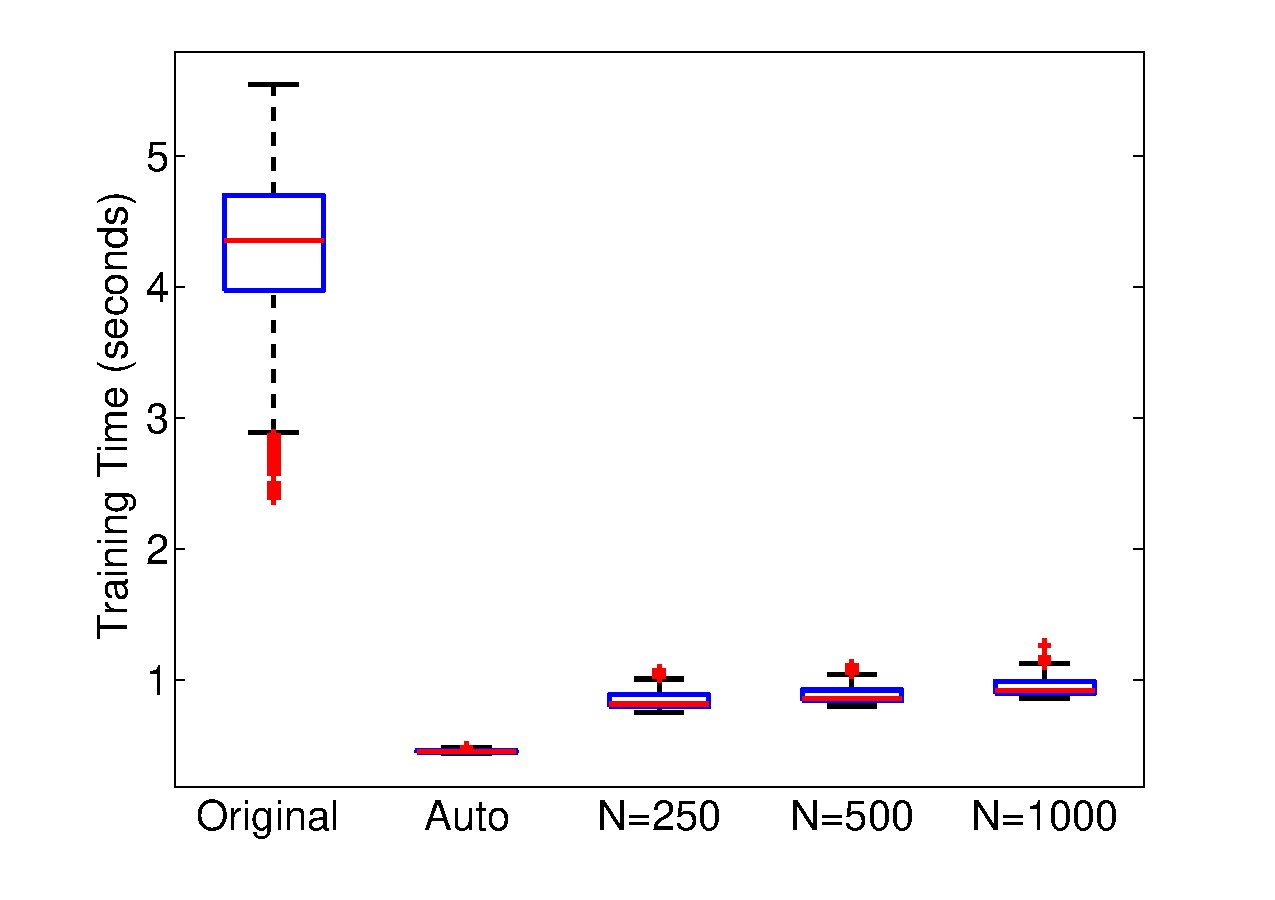
\includegraphics[width=0.33\columnwidth]{box_plot_path_time} \label{fig:pathfinder_tr_times_boxplots}}
	%pathfinder_errors_boxplot_2012_all_models_night.pdf
	%pathfinder_tr_times_boxplot_2012_all_models_night   
	\caption{Performance of the kernel observer over AVVHR satellite 2012 data with different numbers of observation locations.}
\end{figure}

\begin{figure*}
    \centering
    \hspace{-0.3in}\subfloat[6th May]{
	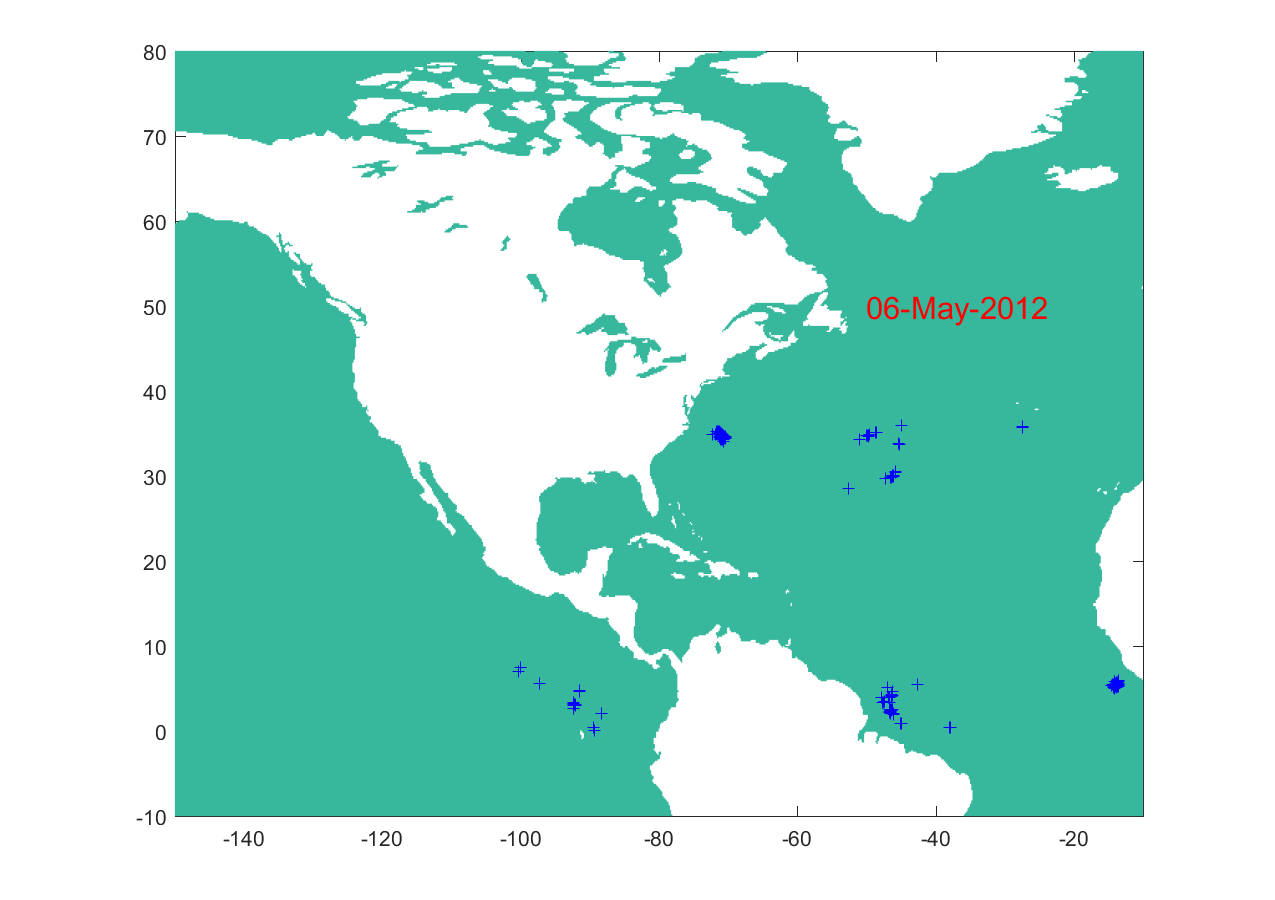
\includegraphics[scale=0.22]{May6}
	\label{fig:May6 } }
	\hspace{-0.5in}
	\subfloat[7th May]{
	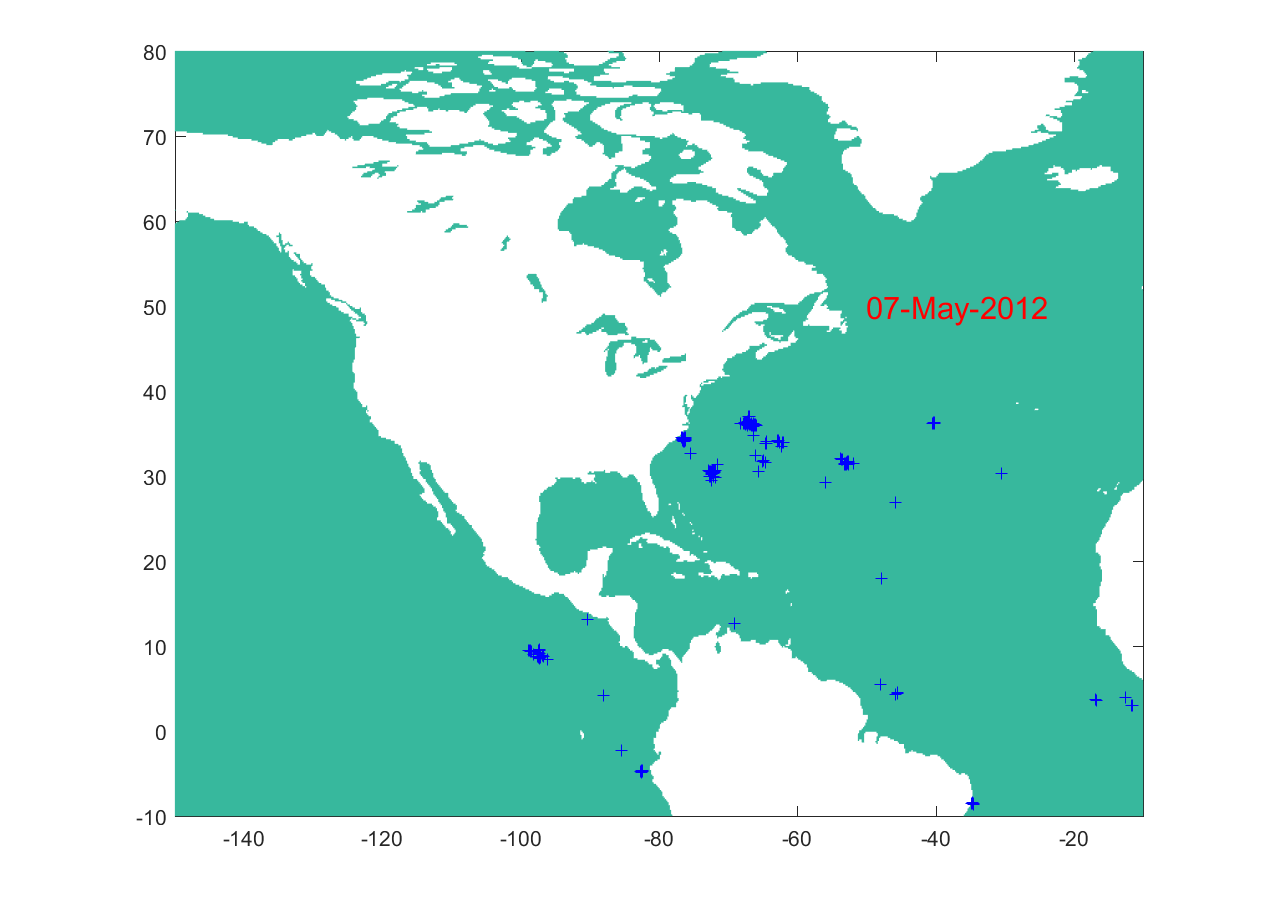
\includegraphics[scale=0.22]{May7}
	\label{fig:May7 } }
	\hspace{-0.5in}
	\subfloat[28th May]{
	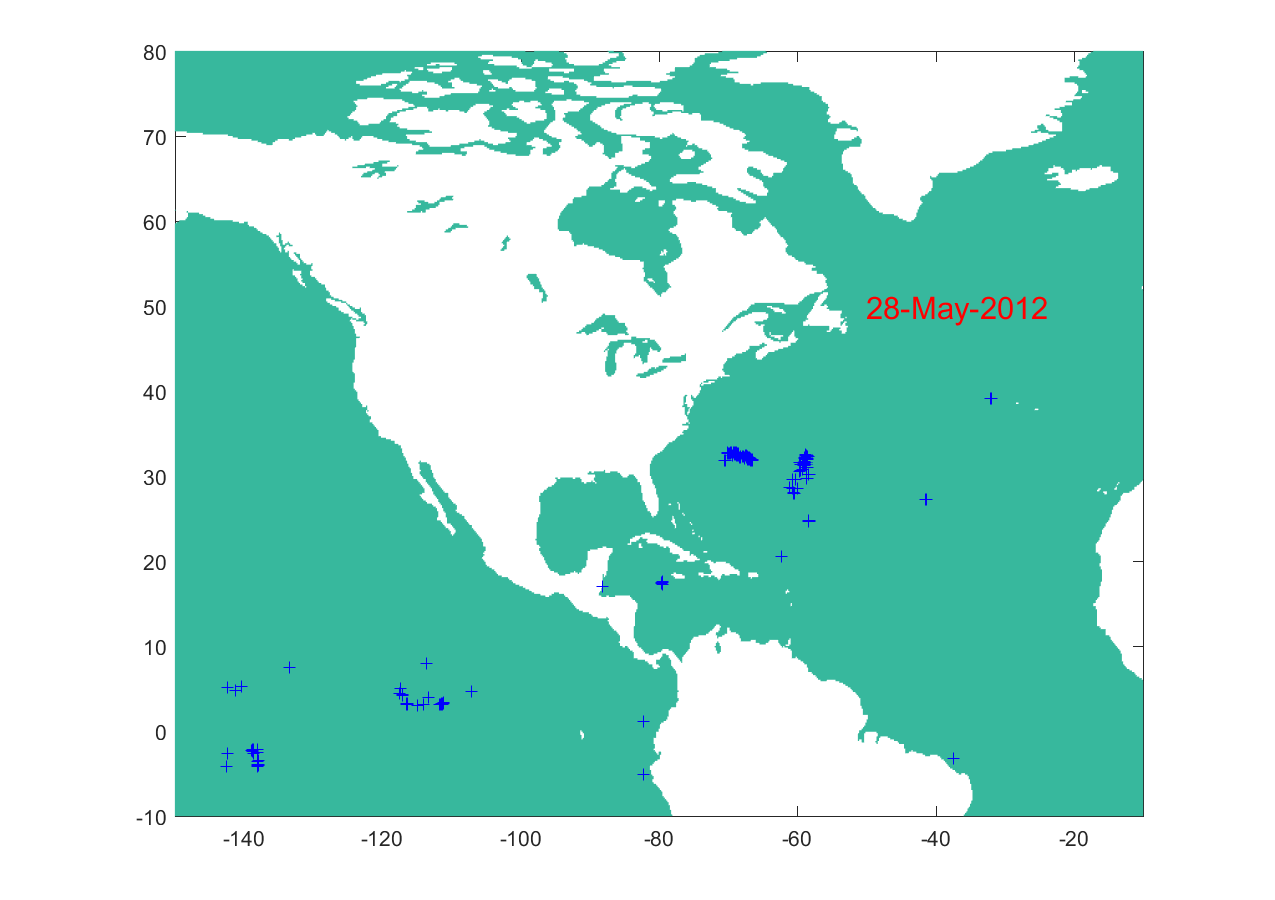
\includegraphics[scale=0.22]{May28}
	\label{fig:May28 } }
	\hspace{-0.5in}\subfloat[29th May]{
	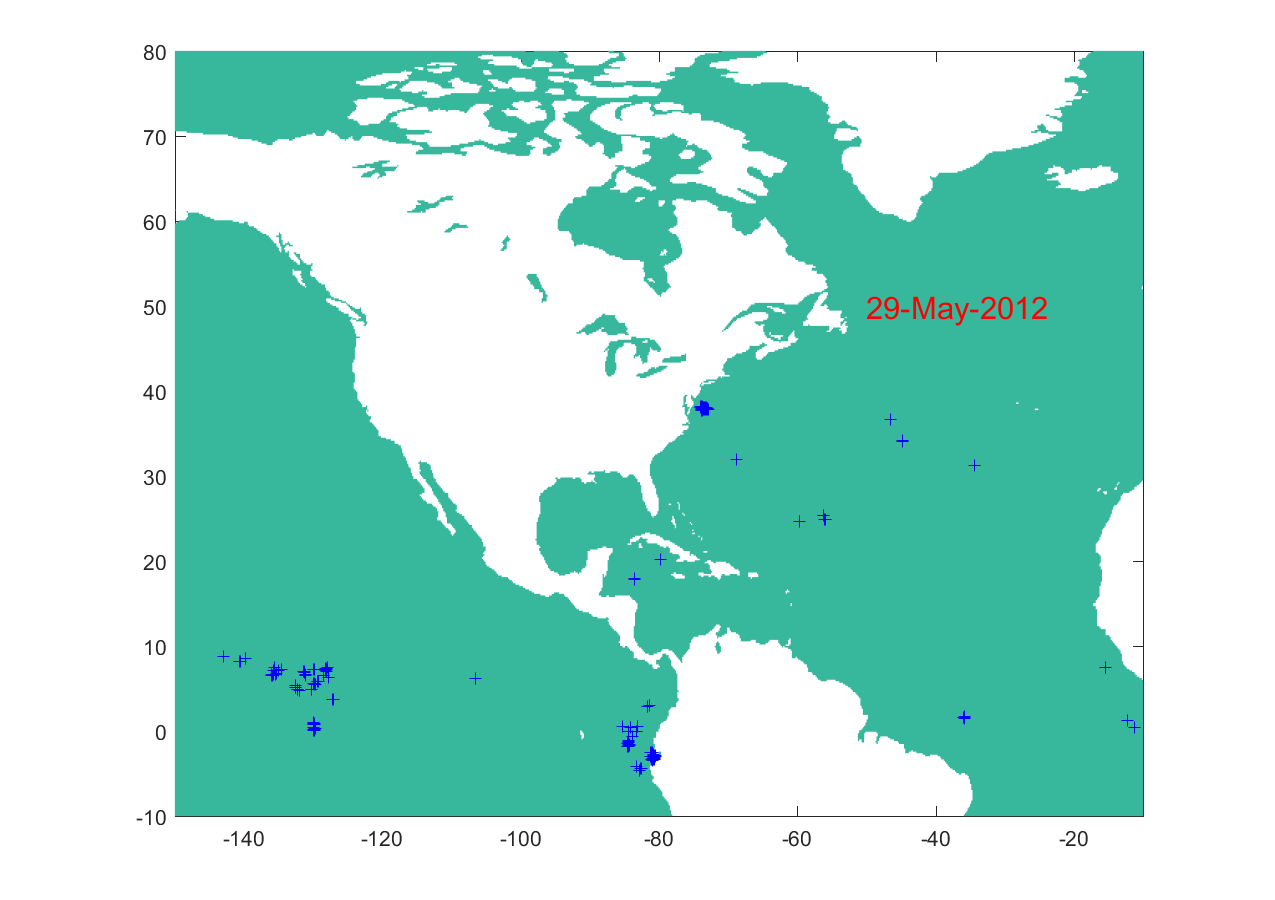
\includegraphics[scale=0.22]{May29}
	\label{fig:May29 } }
	\caption{Locations of weather anomaly obtained based on the error between the acutual temperature and the prediction of autonomous kernel observer. Landmass is shown in white and the ocean is in green. Locations marked have error greater than two standard deviations above the mean error. }
	\label{fig:anomaly}
\end{figure*}

\subsection{Predicting evolution of weed density in agricultural fields}\label{sec:weed}

\subsection{Control of a linear PDE} %with AVHRR Satellite data}
We then employed kernel controllers for controlling an approximation to the scalar diffusion equation $u_t = bu_{xx}$ on the domain $\dom=[0,1]$, with $b=0.25$. The solution to this equation is infinite-dimensional, so we chose a kernel $\kernel(x,y) = e^{-(\|x-y\|^2/2\s^2)}$, and a set of atoms  $\Atoms=\shCentLong$, $c_i\in\dom$, with $\ncent = 25$ generating $\fspaceC$, the space approximating $\fspace$, and another set of atoms $\AtomsControl=\{\fmap(d_1),\dots,\fmap(d_{\ncontrol})\}$, $d_j\in\dom$,
$\ncontrol=13$, generating the control space $\fspaceD$. The number of, and the location of the observations was chosen to be the same as that of the actuation locations $d_j$. First, tests (not reported here) were conducted to ensure that the solution to the diffusion equation is well approximated in $\fspaceC$. Matrix least-squares was used to infer $\estsysop$. Figure \ref{fig:uncontrolled_pde} shows an example of an initial function $f_{\text{init}}$ evolving according to the PDE.  A reference function $f_{\text{ref}}\in\fspaceC$ was chosen to drive $f_{\text{init}}$ to $f_{\text{ref}}$ under the action of the PDE. Finally, Algorithm \ref{alg:egp_control} was used to control the PDE, driving $f_{\text{init}}$ to $f_{\text{ref}}$; Figure \ref{fig:controlled_pde_error} shows the absolute value of the error between $f_k $ and $f_{\text{ref}}$ as a function of time. 

% We performed experiments to evaluate the number of randomly placed Actuators and Sensors required as compared to the lower bound obtained in Proposition \ref{prop:2}. Results in Table \ref{compare} shows that randomly placing the sensors and actuators works efficiently for lower set of atoms $ \ncent$ in $ \Atoms$.
% 
% \begin{table}
% 	\caption{Number of randomly placed Actuators and Sensors (average $\pm$ variance) required as compared to the lower bound $\minmeas$ obtained in Proposition \ref{prop:2}. }
% 	\label{compare}
% 	\begin{center}
% 		\begin{tabular}{|c||c||c||c|}
% 			\hline
% 			Set of & Lower  & Number of   & Number of  \\
% 			Atoms & bound ($\minmeas$) & Actuators  &  Sensors \\
% 			
% 			\hline
% 			M = 25 & 10 & 10.27 $\pm$ 0.45 & 10.36 $\pm$ 0.50 \\
% 			M = 30 & 13  & 15.26 $\pm$ 0.51 & 15.24 $\pm$ 0.49 \\
% 			M = 35 & 19  & 21.43 $\pm$ 0.54 & 21.35 $\pm$ 0.50 \\
% 			M = 40 & 24 & 33.08 $\pm$ 6.05 & 32.40 $\pm$ 6.0 \\
% 			% M = 30 & 8.5 $\pm$ 0.8 & 8.5 $\pm$ 0.9 & 10.8 $\pm$ 1.4 \\
% 			\hline
% 		\end{tabular}
% 	\end{center}
% \end{table}

\begin{figure}[tbh] %{r}{0.5\textwidth}
    \centering
    \subfloat[Evolution of initial function $f_{\text{init}}$ according to diffusion equation.]{
    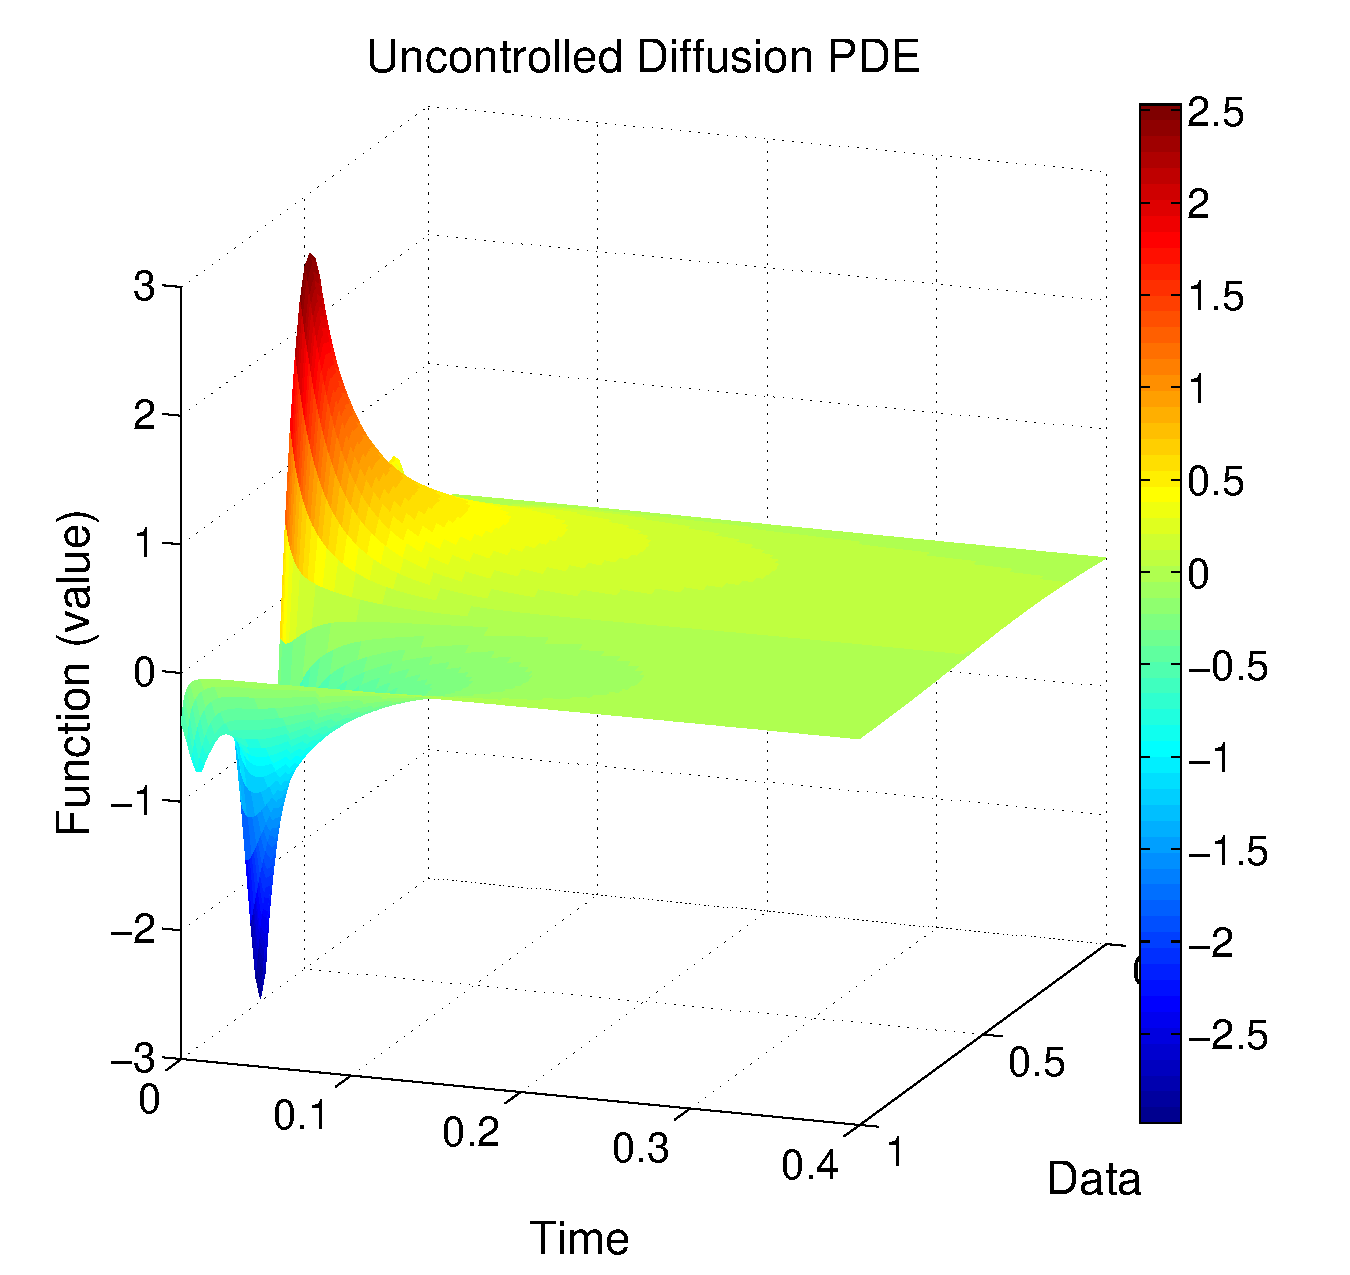
\includegraphics[width=0.45\columnwidth]{uncontrolled_pde_heat.pdf} 
    \label{fig:uncontrolled_pde}}
%     \subfloat[Initial function $f_{\text{init}}$ driven to $f_{\text{ref}}$ using kernel controller.]
%     {
%     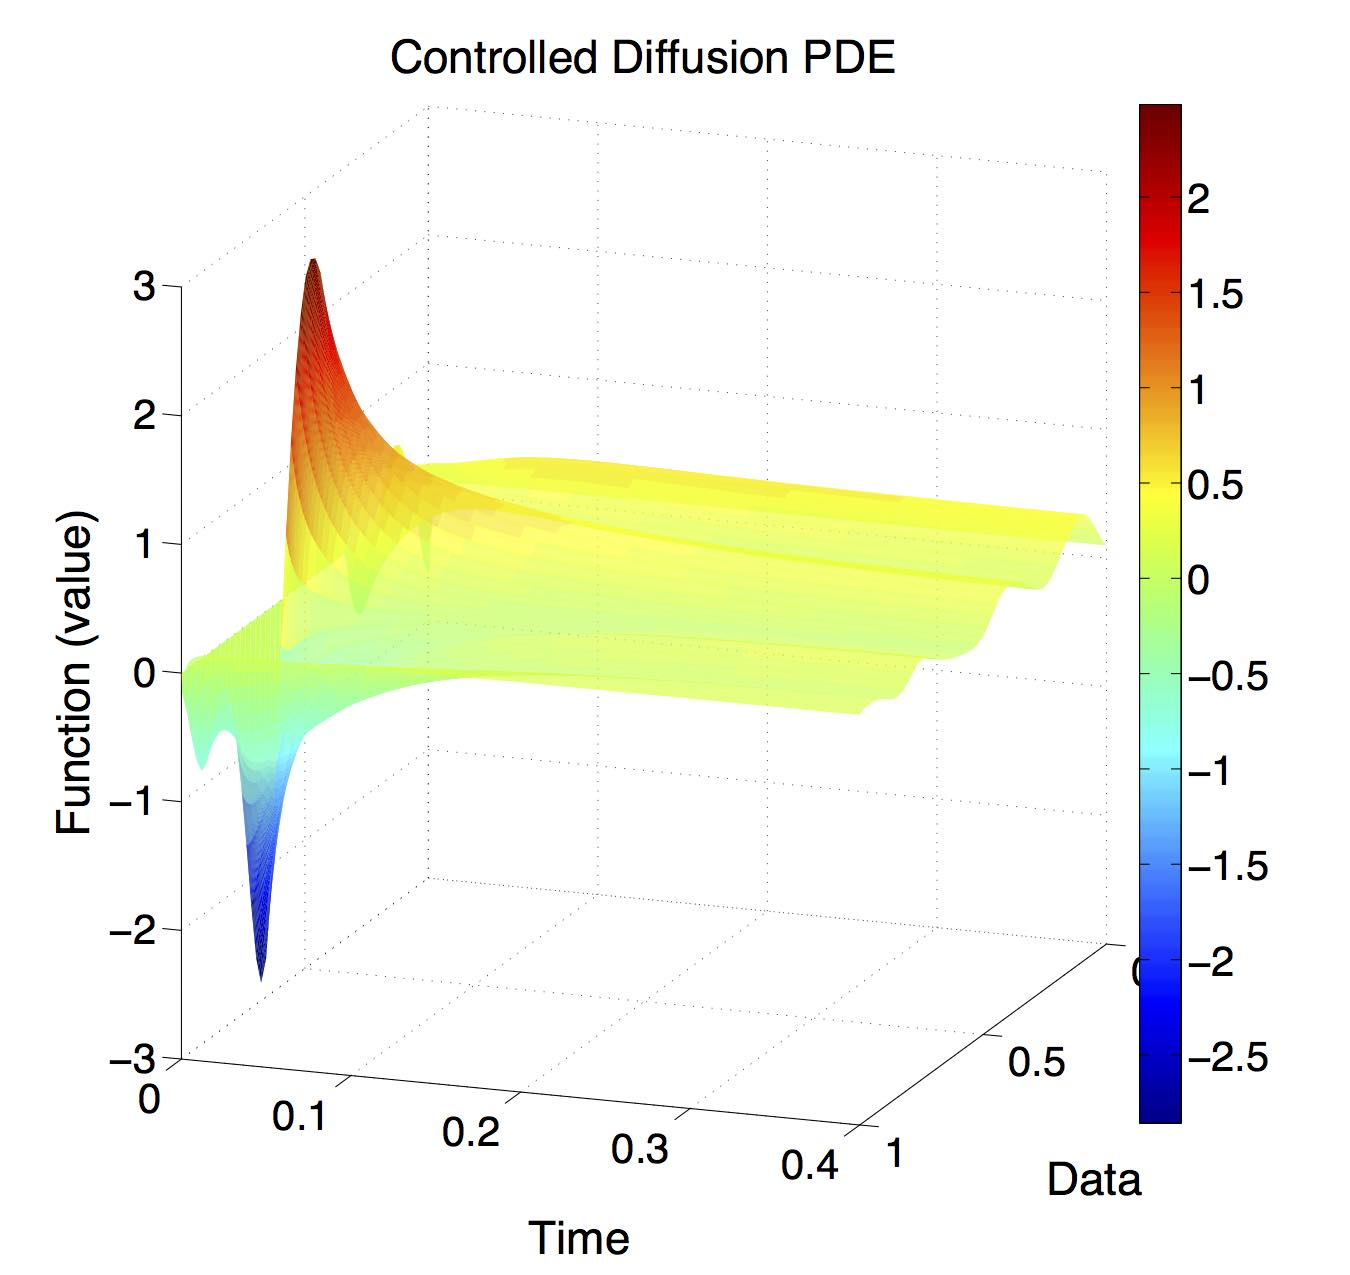
\includegraphics[width=0.5\columnwidth]{controlled_pde_heat.jpg} 
%     \label{fig:controlled_pde}}    
%     \\
    \subfloat[Error in absolute value between controlled pde and $f_{\text{ref}}$. ]{
    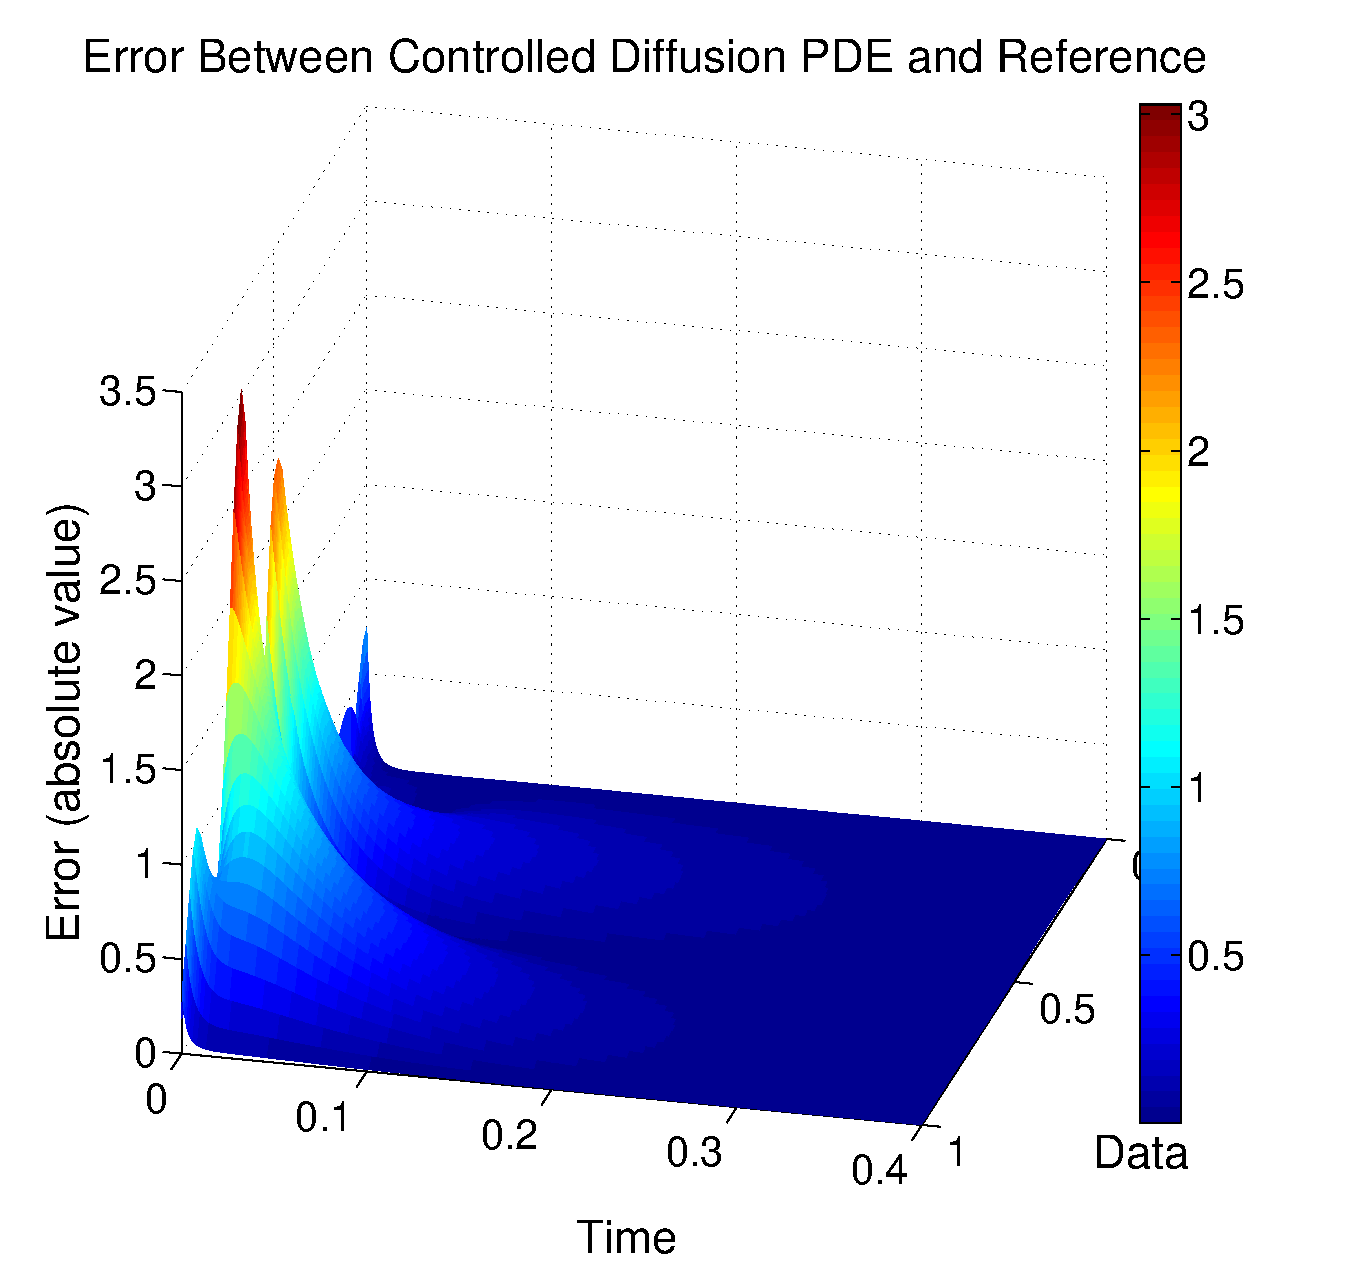
\includegraphics[width=0.45\columnwidth]{controlled_pde_error_heat.pdf} 
    \label{fig:controlled_pde_error} }
    \caption{Demonstration of the control of a linear diffusion equation.}     
\end{figure} 
